\documentclass[12pt]{pwrdpl}

\author{Bartosz Błyszcz}
\shortauthor{B. Błyszcz}

\titlePL{Wykorzystanie algorytmów genetycznych w systemach wykrywania intruzów w sieciach komputerowych}

\shorttitlePL{Wykorzystanie algorytmów genetycznych w systemach wykrywania intruzów}

\thesistype{PRACA DYPLOMOWA\\\vspace*{1mm}MAGISTERSKA}

\supervisor{dr inż. Tomasz Babczyński}

\degreeprogramme{Informatyka Techniczna}

\date{2024}

\faculty{Wydział Informatyki i Telekomunikacji}

\begin{document}

	\titlepages
	\RedefinePlainStyle
	
	\setcounter{tocdepth}{2}
	\tableofcontents
	\clearpage
	\section*{Wykaz skrótów}

\begin{table}[H]
    \centering
    \begin{tabularx}{\linewidth}{lXX}
        \textbf{Skrót} & \textbf{Nazwa angielska} & \textbf{Nazwa polska} \\ \hline
        \textbf{GA} & \textit{Genetic Algorithm} & Algorytm Genetyczny \\ \hline
        \textbf{GP} & \textit{Genetic Programming} & Programowanie Genetyczne \\ \hline
        \textbf{IDS} & \textit{Intrusion Detection System} & System wykrywania intruzów  \\ \hline
        \textbf{IPS} & \textit{Intrusion Prevent System} & System zapobiegania włamaniom \\ \hline
        \textbf{GNB} & \textit{Gaussian Naive Bayes} & Naiwny Klasyfikator Bayesa wykorzystujący rozkład Gaussa \\ \hline
        \textbf{ANN} & \textit{Artificial Neural Network} & Sztuczna sieć neuronowa \\ \hline
        \textbf{CNN} & \textit{Convolutional Neural Network} & Konwolucyjna sieć neuronowa \\ \hline
        \textbf{ML} & \textit{Machine Learning} & Uczenie maszynowe \\ \hline
        \textbf{AI} & \textit{Artificial Intelligence} & Sztuczna Inteligencja \\ \hline
        \textbf{IDS} & \textit{Intrusion Detection System} & System Wykrywania Intruzów \\ \hline
        \textbf{SVM} & \textit{Support Vector Machine} & Maszyna Wektorów Nośnych \\ \hline
        \textbf{AUC} & \textit{Area Under Roc Curve} & Przestrzeń pod krzywą ROC \\ \hline
        \textbf{LCDPs} & \textit{Low-code Development Platforms} & Platforma Low-code \\ \hline
        \textbf{BI} & \textit{Business Intelligence} & Narzędzia biznesowe do~przekształcania danych \\ \hline
        \textbf{CDN} & \textit{Content Delivery Network} & Sieć dostarczania zawartości \\ \hline
        \textbf{MLP} & \textit{Multilayer Perceptron network} & Sieć wielowarstwowa perceptronowa \\ \hline
        \textbf{Azure ML} & \textit{Azure Machine Learning Studio} & Azure Machine Learning Studio \\ \hline
        \textbf{GAGNB} & \textit{Gaussian Naive Bayes - with GA} & Gaussian Naive Bayes - with GA\\ \hline
        \textbf{HTTPS} & \textit{Hyper Text Transfer Protocol Secure} & Protokół służący do komunikacji w sieci internetowej \\ \hline
        \textbf{REST} & \textit{Representative State Transfer} & Rozwiązanie architektoniczne służące do komunikacji w sieci internetowej \\ \hline
    \end{tabularx}
    \label{tab:shorts}
\end{table}
	
	\sloppy
	\setnowidow
	
	\chapter{Wstęp}

\section{Wprowadzenie i uzasadnienie tematu pracy}
Klasyfikacja danych tabelarycznych jest trudnym zagadnieniem do analizy, z powodu powszechnego występowania bardzo dużej ilości nieuporządkowanych danych, które zawierają wiele cech.\ To proces organizowania danych w tabeli w celu ich łatwiejszej analizy, interpretacji czy dalszego przetwarzania.\ Podczas takiej kategoryzacji danych ważne jest właściwe dobranie algorytmu, ze względu na typ danych.\ Przykładowo zbiór danych tekstowych można klasyfikować za pomocą jednokierunkowej sieci neuronowej, a obrazy za pomocą sieci konwolucyjnej.\
\\ \\
Obecnie istnieje wiele różnych algorytmów do klasyfikacji danych tabelarycznych.\ Jednymi z popularniejszych są: regresja logistyczna \trans{ang. logistic regression}, drzewo decyzyjne \trans{ang. decision tree}, las losowy \trans{ang. random forest}, maszyna wektorów nośnych \trans{ang. support vector machine}, naiwny klasyfikator Bayesowski \trans{ang. Naive Bayes classifier}.\ Przy wykorzystaniu tych algorytmów do kategoryzacji, ważne jest właściwe wybranie algorytmu, czyli rozpoznanie z jakimi danymi mamy do czynienia oraz porównanie wyników klasyfikacji, w celu wybrania najlepszego dopasowania.
\\ \\
Dane tabelaryczne występują w każdej dziedzinie, duże zestawy danych można spotkać w medycynie, nauce czy w finansach.\ Rosnąca liczba danych oraz ich zmienna struktura wymaga opracowywania coraz lepszych algorytmów klasyfikacji.\ Jednakże wyjątkowość danych sprawia, że trudno opracować uniwersalny algorytm klasyfikacji.\ Wiele rozwiązań jest tworzonych dla konkretnej struktury danych, co powoduje niemożność ich wykorzystania dla innych danych.
\\ \\
Przy rosnącej liczbie danych do analizy, rozwijają się metody ułatwiające ich klasyfikację. Coraz częściej wykorzystuje się rozwiązania z zakresu sztucznej inteligencji czy obliczeń chmurowych. Jednym z przykładów jest aplikacja \textit{Machine Learning Studio},  dostarczana przez \textit{Microsoft Azure}. Zawiera ona zestaw narzędzi, umożliwiających łatwiejsze kategoryzowanie danych czy tworzenie algorytmów klasyfikacji i ich porównywanie. Użycie chmury pozwala na wykorzystanie mocy obliczeniowej sklasteryzowanych jednostek wirtualnych do wykonywania obliczeń na odpowiednich maszynach wirtualnych czy do budowania skomplikowanych zautomatyzowanych procesów złożonych z wielu zadań \trans{ang. pipeline}. Natomiast wykorzystanie sztucznej inteligencji pozwala na wprowadzenie elementu uczenia się w celu lepszego rozpoznawania danych.
\\ \\
Zastosowanie tych narzędzi umożliwia automatyzację procesu badawczego, porównanie wyników działania różnych algorytmów oraz znaczne przyspieszenie badań.\ Ma to znaczenie przy rosnącym zaprotrzebowaniu na analizę dużych zestawów danych.
\\ \\
W dobie rozwijających się hurtowni danych oraz sztucznej inteligencji coraz więcej firm przetrzymuje ogromne zbiory danych w sieci komputerowej.\ Dane takie mogą być poufne bądź o znaczeniu strategicznym.\ Wyciek takich danych może mieć negatywne konsekwencje dla właścicieli danych bądź osób, których dane sa przechowywane.\ Przykładem może być dostęp do prywatnych kont bankowych albo danych medycznych.\ Dlatego też dane te są zabezpieczane m.in. przy użyciu kryptografii.\ Pozwala to na zaszyfrowanie przesyłu danych poufnych jak i samych przesyłanych danych.\ Jednakże osobom planującym kradzież konkretnych danych dużo bardziej zależy na uzyskanie nieautoryzowanego dostępu do komputerów mogących posiadać dostęp do danych wrażliwych.\ Dzieje się tak, ponieważ dostęp do urządzeń, pozwala na wgląd nie tylko do konkretnych danych ale i do całej sieci intranetowej np. banku.\ Dostęp taki może zostać również wykorzystany do np. wgrania szkodliwego oprogramowania umożliwiającej założenie ,,\textit{tylnej furtki}'' \textit{(ang. backdoor)}.\ W celu ograniczenia możliwych nieautoryzowanych dostępów z zewnątrz powstało oprogramowanie \textit{IDS, IPS} \textit{(ang. Intrusion Detection system, Intrusion Prevent System)}.\ Systemy do ostrzegania i przeciwdziałania atakom na sieć komputerową~\cite{Blyszcz2022}.
\\ \\
Dane sieciowe są bardzo złożone oraz posiadają dużo cech, dlatego do ich analizy można wykorzystać algorytmy uczenia maszynowego pozwalające na wykrycie nietypowego ruchu sieciowego.\ Klasyczne systemy IDS bazują głównie na regułach wykluczających konkretny ruch sieciowy.\ Przewagą uczenia maszynowego jest to, że może wykrywać anomalie niewchodzące w skład reguł bezpieczeństwa w sieci.\ Może to umożliwić przy niewielkim koszcie wytrenowania sieci wczesne i szybsze wykrywanie potencjalnych ataków niż w przypadku klasycznyc hsystemów IDS opartych o reguły.

\section{Cel i zakres pracy}
Celem niniejszej pracy dyplomowej jest ocena jakości opracowanego w pracy inżynierskiej autorskiego sposobu klasyfikacji danych tabelarycznych, wykorzystującego algorytm genetyczny oraz Klasyfikator Naiwny Bayesa.\ W tym celu dokonano analizy porównawczej rozwiązania wraz z algorytmami dostępnymi w aplikacji \textit{Machine Learning Studio}. Algorytmy opisano w Podrozdziale~\ref{sec:alg}.
\\ \\
Praca składa się z 2 części.\ W części teoretycznej (Rozdziały 2 - 5) dokonano przeglądu dostępnych rozwiązań chmurowych (podejścia low-code/no-code).\ Oprócz tego opisano zagadnienia związane ze sztuczną inteligencją.\ W części badawczej (Rozdziały 6 - 8) przygotowano programistyczne stanowisko badawcze.\ W tym celu scharakteryzowano metryki jakościowe i opracowano eksperyment.\ Wykonano analizę porównawczą i statystyczną otrzymanych wyników.\ Dane wykorzystane do badań pochodziły z Instytutu Cyberbezpieczeństwa, działającego przy Uniwersytecie Nowy Brunszwik.


	\chapter{Sieci neuronowe}
	\chapter{Klasyfikacja danych}

 Człowiek od zawsze próbuje skategoryzować i uporządkować posiadaną wiedzę w zbiory pozwalające na łatwy dostęp do przechowywanych informacji na przykład w sposób tabelaryczny. Klasyfikacja to proces rozpoznawania obiektów na bazie analizy ich cech. Jest to jedna z pierwszych rzeczy, której uczą się niemowlęta: rozróżniania kształtów, kolorów czy własnych rodziców. \ W póżniejszych latach te umiejętności są bardzo ważne, ponieważ w otaczającym świecie wiele rzeczy jest sklasyfikowanych. Przykładem takiej klasyfikacji są książki w katalogach bibliotecznych czy produkty spożywcze według jakości produkcji.
\\ \\
W uczeniu maszynowym klasyfikacja jest to metoda uczenia nadzorowanego, podczas której model próbuje przewidzieć etykietę obiektu na podstawie jego cech. Proces uczenia modelu klasyfikacji jest oparty o dwa zbiory, treningowy i testowy. Zbiór treningowy powinien być mniejszy od zbioru testowego. Po udanym procesie trenowania modelu następuje proces testowania, na podstawie którego wylicza się odpowiednie metryki pozwalające na ewaluacje modelu. W pracy magisterskiej wykorzystano zbiór danych, który posiada dwa typy etykiet [0, 1], dlatego też na tej podstawie zbudowano macierz pomyłek.

\section{Metryki klasyfikacji danych}
W trakcie ewaluacji algorytmu służącego do klasyfikacji wykorzystuje się metryki klasyfikacji. Służą one do przewidywania etykiet klas na podstawie danych wejściowych. W zależności od ilości klas wyjściowych rozróżniamy klasyfikację binarną i wieloklasową. W klasyfikacji binarnej występują tylko dwie klasy wyjściowe, a w klasyfikacji wieloklasowej już tych klas jest więcej. Przykładem klasyfikacji binarnej jest np. wykrywanie niechcianych wiadomości w skrzynce mailowej. Wiadomość przychodzącą możemy określić jako 1 - \textit{,,pozytywną''}, bądź 0 - \textit{,,negatywną''}. Istnieje wiele sposobów na oceny klasyfikacji, do których zaliczamy między innymi dokładność, macierz pomyłek czy precyzję~\cite{Agrawal2024}.
\\ \\
Macierz pomyłek pokazuje jakie wyniki możemy otrzymać w procesie klasyfikacji. \refsource{Tabela}{tab:matrix-tn} obrazuje schemat macierzy pomyłek. Jest to miara wydajności problemów klasyfikacji.

\begin{table}[H]
    \centering
    \captionsource{Macierz pomyłek}{Opracowanie własne}
    \label{tab:matrix-tn}
    \begin{tabular}{|c|c|M{16mm}|M{16mm}|}
        \hline
         & & \multicolumn{2}{c|}{\textbf{Prawdziwe wartości}} \\ \hline
         & & \textbf{1} & \textbf{0} \\ \hline
        \rule{0pt}{13mm} \multirow{2}{*}{\rotatebox[origin=c]{90}{\parbox{18mm}{\textbf{Przewidziane wartości}}}} & \textbf{1} & \cellcolor{lightgreen}TP & \cellcolor{lightred}FN \\ \cline{2-4}
        \rule{0pt}{13mm} & \textbf{0} & \cellcolor{lightred}FP & \cellcolor{lightgreen}TN \\ \hline
    \end{tabular}
\end{table}
    Wyróżniamy 4 rodzaje rezultatów:
    \begin{itemize}
        \item  \textbf{TP} (\textit{prawdziwie pozytywny}) -- przewidywano pozytywny wynik i otrzymano pozytywny wynik,
        \item \textbf{FN} (\textit{fałszywie negatywny}) -- przewidywano negatywny wynik, a otrzymano pozytywny wynik,
        \item \textbf{FP} (\textit{fałszywie pozytywny}) -- przewidywano pozytywny wynik, a otrzymano negatywny wynik,
        \item \textbf{TN} (\textit{prawdziwie negatywny}) -- przewidywano negatywny wynik i otrzymano negatywny wynik.
    \end{itemize}

Opierając się o macierz pomyłek można wyznaczyć następujące metryki:
\begin{itemize}
    \item dokładność,
    \item precyzję,
    \item czułość,
    \item F1
    \item swoistość
    \item ROC-AUC~\cite{Agrawal2024}
\end{itemize}

\subsection{Dokładność}
\begin{equation}\label{math:acc}
    \frac{TP + TN}{TP + TN + FP + FN}
\end{equation}
Dokładność określa częstość poprawnego przewidywania klasyfikatora. Jest to stosunek wszystkich dobrze oznaczonych obiektów do liczby wszystkich prób~\cite{Agrawal2024, Blyszcz2022, Kulkarni2020}.

\subsection{Precyzja}
\begin{equation}\label{math:prec}
    \frac{TP}{TP + FP}
\end{equation}
Precyzja wyjaśnia ile z prawidłowo przewidzianych przypadków jest poprawnych. Jest to stosunek poprawnie wybranych obiektów klasy ,,\textit{1}'', do wszystkich wybranych obiektów tej klasy. Znajduje zastosowanie w przypadkach gdy wynik fałszywie dodatni jest większym problemem niż fałszywie ujemny~\cite{Agrawal2024, Blyszcz2022, Kulkarni2020}.

\subsection{Czułość}
\begin{equation}\label{math:rec}
    \frac{TP}{TP + FN}
\end{equation}
Czułość określia ile rzeczywistych pozytywnych przypadków byliśmy w stanie poprawnie przewidzieć za pomocą naszego modelu. Jest to stosunek poprawnie sklasyfikowanych obiektów klasy ,,\textit{1}'', do wszystkich obiektów, które powinny być w tej klasie. Czułość jest przydatną metryką w przypadkach gdy wynik fałszywie ujemny ma większe znaczenie niż wynik fałszywie dodatni~\cite{Agrawal2024, Blyszcz2022, Kulkarni2020}.

\subsection{Swoistość}
\begin{equation}\label{math:swo}
    \frac{TN}{TN + FP}
\end{equation}
Swoistość lub specyficzność pozwala określić ile rzeczywiście uzyskało się przypadków negatywnych. Jest to stosunek poprawnie zaklasyfikowanych obiektów klasy ,,\textit{0}'', do wszystkich obiektów, które powinny być w tej klasie~\cite{Agrawal2024}.

\subsection{F1}
\begin{equation}\label{math:f1}
   \frac{2*x*y}{x + y}
\end{equation}
Parametr F1 pozwala na połączoną ocenę precyzji i czułości. Jest to średnia harmoniczna precyzji (\textit{x}) i czułości (\textit{y}). Parametr F1 może być skuteczną metryką oceny w następujących przypadkach:
\begin{itemize}
    \item wyniki fałszywie pozytywne i fałszywie negatywne są równie kosztowne
    \item zwiększenie ilości danych nie zmienia skuteczności wyniku
    \item wynik prawdziwie ujemny jest wysoki~\cite{Agrawal2024}.
\end{itemize}

\subsection{ROC - AUC}
Krzywa ROC-AUC przedstawiona na \refsource{rysunku}{fig:roc-auc}, pozwala na ocenę sprawności klasyfikatora. ROC jest krzywą prawdopodobieństwa, którą wykreśla czułość w stosunku do swoistości. Wykres przedstawia wydajność (dokładność predykcji) modelu klasyfikacji. AUC \textit{(ang. Area Under Roc Curve)} jest to pole pod krzywą ROC. AUC to miara zdolności klasyfikatora do rozróżniania klas.

\begin{figure}[H]
    \centering
    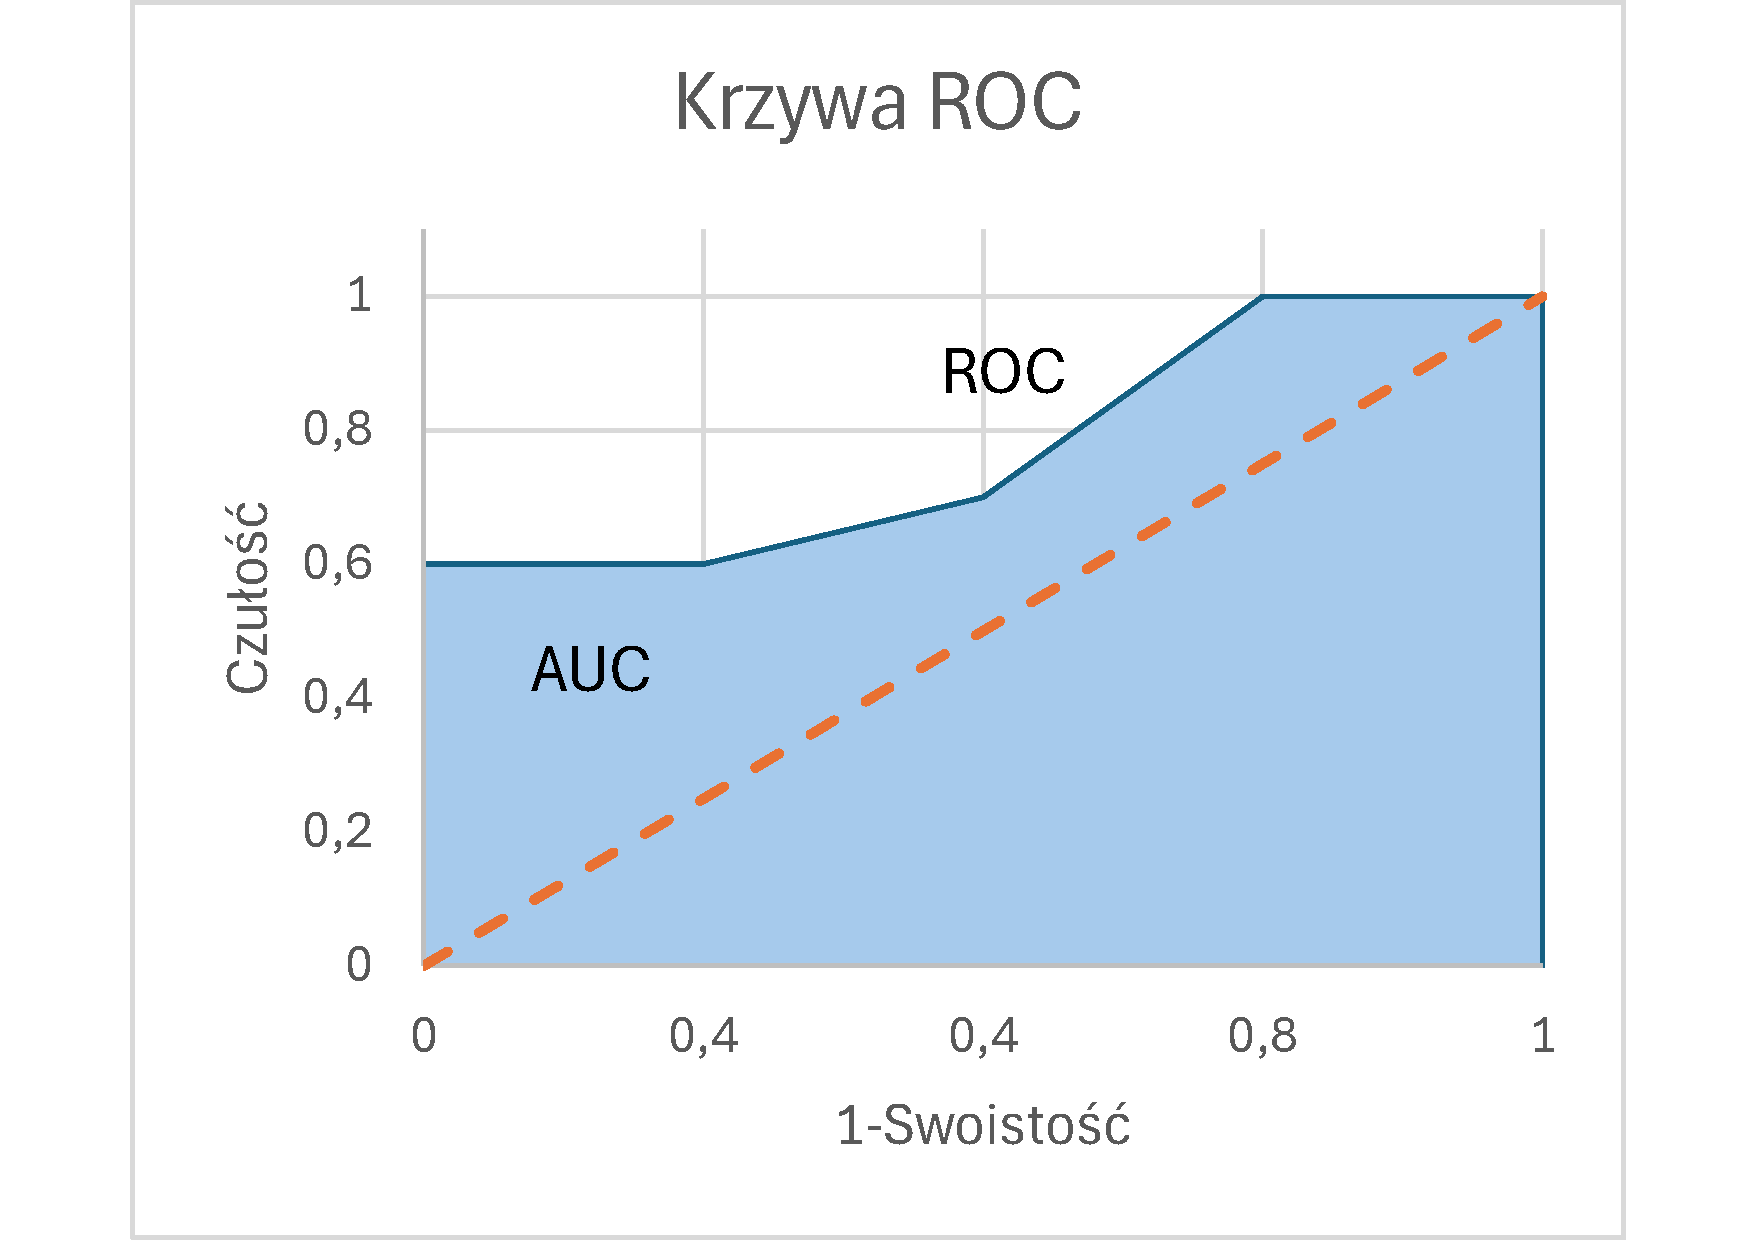
\includegraphics[width=0.8\textwidth]{images/roc-auc}
    \captionsource{Przykład krzywej ROC}{Opracowanie własne}
    \label{fig:roc-auc}
\end{figure}

Im większa jest wartość AUC tym lepsza wydajność modelu w rozróżnianiu klas pozytywnych i negatywnych. Wynik AUC jest z zakresu $[0, 1]$:
\begin{itemize}
    \item AUC = 1 -- klasyfikator idealny, który rozróżnia wszystkie punkty,
    \item 0,5 < AUC < 1 -- klasyfikator prawie idealny, czyli z dużym prawdopodobieństwem sklasyfikuje poprawnie obiekty
    \item AUC = 0,5 -- klasyfikator losowy, oznacza to, że nie ma pewności czy klasyfikator jest w stanie rozpoznać cechy, czy może przypisuje je losowo,
    \item AUC < 0,5 -- klasyfikator gorszy niż klasyfikator losowy~\cite{Algolytics, Agrawal2024}.
\end{itemize}
	\chapter{Podejście low-code/no-code}
Low-Code oraz no-code to nowe podejście skupiające się na umożliwieniu tworzenia programów w sposób nie wymagający znajomości języka oprogramowania. Podejście to ma pozwolić osobom nie będącymi programistami na tworzenie aplikacji biznesowych. Ma to zwiększyć tempo tworzenia rozwiązań biznesowych, na które zapotrzebowanie wciąż rośnie. Jednakże podejście to jest stosounkowo świeżym podejściem, którego początki można było obserwować w codziennym życiu na przykład podczas tworzenia stron internetowych korzystając z narzędzi takich jak \textit{Wordpress}, \textit{Joomla}, \textit{Wix}. Narzędzia te umożliwiają w łatwy sposób tworzyć stronę z tak zwanych kafelków, które umieszczone w odpowiednim miejscu były odpowiedzialne za jedną konkretną rzecz\cite{Wordpress2023, Joomla2023, Wix2023}. Przykład na \refsource{obrazie}{fig:pa-plat}, \textbf{\ref{fig:wp-plat}}.
\begin{figure}[H]
    \centering
    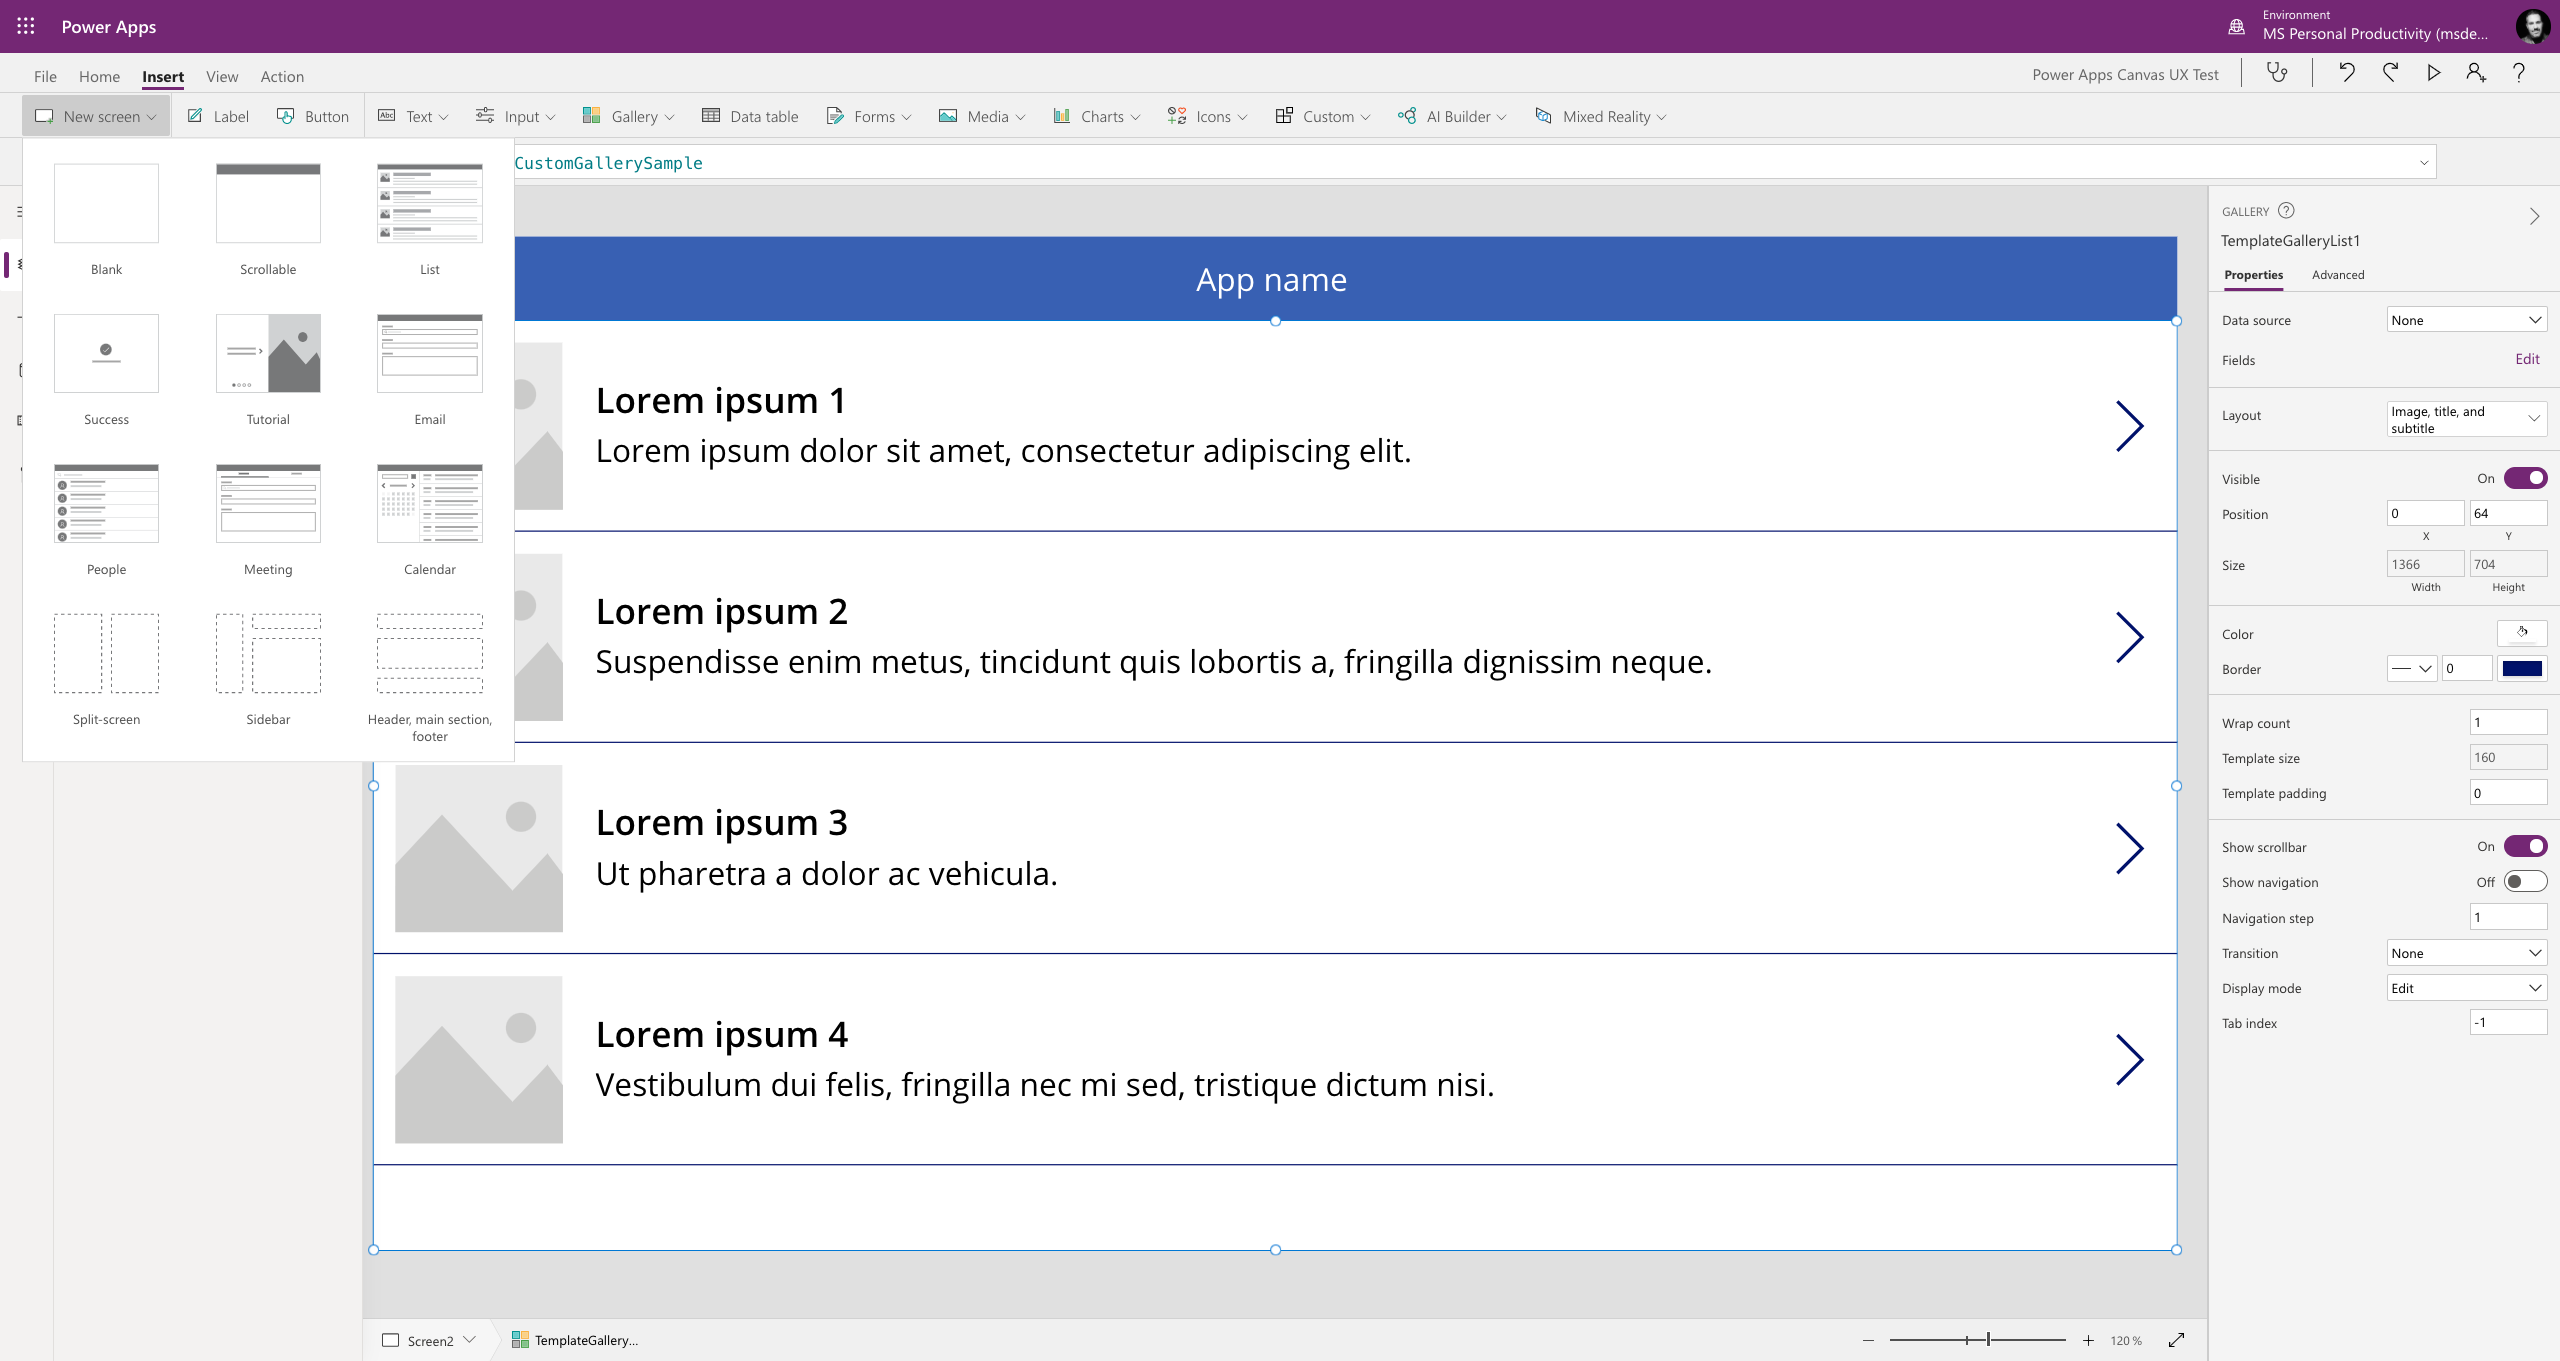
\includegraphics[width=0.6\textwidth]{images/ms_powerapps}
    \captionsource{PowerApps od Microsoft}{\cite{Powerapps2023}}
    \label{fig:pa-plat}
\end{figure}

\begin{figure}[H]
    \centering
    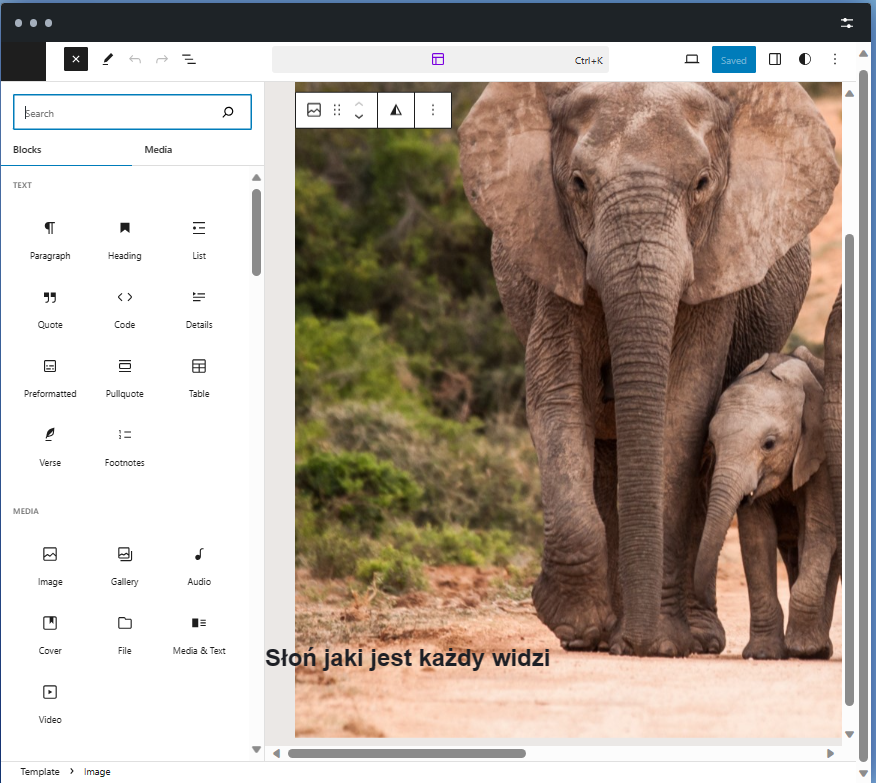
\includegraphics[width=0.4\textwidth]{images/slon_wordpress}
    \captionsource{Wordpress.com}{\cite{WordpressDeveloper2023}}
    \label{fig:wp-plat}
\end{figure}

Coraz większa popularnością cieszą się platformy low-code\trans{ang. Low-code Development Platforms} (\textbf{LCDPs}) dostarczane między innymi przez Google, Microsoft, Amazon pozwalają one na tworzenie wysoko skalowalnych rozwiązań przy niewielkim albo i żadnym nakładzie programowania. Ma to umożliwić osobom z niewielkim doświadczeniem w programowaniu, na szybkie wdrożenie oraz tworzenie niezawodnego oprogramowania. Twórcy platform oferują również korzystającym zmniejszenie ilości pracy potrzebnej do wdrożenia albo rozwijania kolejnych funkcjonalności\cite{Bock2021, Hirzel2022}.
\\ \\
\section{Platformy}
LCDP udostępniane twórcom aplikacji, umożliwiają skalowalność rozwiązań tworzonych na własne potrzeby. Dodatkowo są popularne przy tworzeniu aplikacji typu ''\textit{aplikacja jako usługa}'' \trans{ang. Software-as-a-Service} (SaaS), które opłacane są tylko za stopień ich użycia, co w niektórych przypadkach może się okazać dużo bardziej opłacalne niż utrzymywanie swoich rozwiązań serwerowych. Dzięki takim rozwiązaniom wiele małych firm będzie mogło pozwolić sobie na tworzenie i utrzymywanie dostosowanych rozwiązań opartych o ekosytem \textit{Microsoft365} / \textit{Google Workspace}.

\subsection{Microsoft PowerApps}
Jest to platforma programistyczna umożliwiająca tworzenie niestandardowych aplikacji dla rozwiązań biznesowych. Umożliwia ona tworzenie aplikacji opartych o różnorakie źródła danych do których należą między innymi: SQL Server, SharePoint, Dynamics 365. Dodatkową zaletą tego rozwiązania jest tworzenie aplikacji responsywnych, działających dobrze na wielu rodzajach urządzeń. Dodatkowow platforma ta pozwala tworzyć trzy typy aplikacji przy braku konieczności kodowania\cite{Microsoftc}
\begin{itemize}
    \item \textbf{Kanwa} - jest to typ aplikacji oparty o model danych znajdujący się na przykład w Excelu. Aplikację tego typu tworzy się za pomcą przesuwanych kafelek, a proces przypomina po trochu robienie prezentacji przy użyciu aplikacji Powerpoint, co umożliwia pełną dowolność w tworzonym interfejsie graficznym\cite{Microsoftb}.

    \item \textbf{Oparte na modelu} - w ramach korzystania z usługi Microsoft Dataverse można wygenerować aplikacje bazujące na danym modelu danych, przez co użytkownicy otrzymują produkt ułatwiający im analizę danych\cite{Microsofta}.

    \item \textbf{Karty} - są to uproszczone aplikacje, które można dodać do usługi Micrsoft Teams w określonym biznesowym celu. Dużą zaletą tego rozwiązania jest możliwość korzystania z źródeł danych, dzięki czemu poszczególne karty mogą odpowiadać za jedno zadanie biznesowe\cite{Microsoft}.
\end{itemize}

\subsection{Amazon QuickSight}
Jest to rozwiązanie firmy Amazon, które umożliwia firmom dostarczanie rozwiązań z zakresu analityki biznesowe\trans{ang. business intelligence} (BI) dzięki interaktywnym pulpitom korzystającym z jednego źródła prawdy. Dodatkowo korzystanie z interaktywnych formularzy, raportów oraz zapytań w języku naturalnym pozwala interesariuszom otrzymać możliwość korzystania z jednolitych rozwiązań opartych o różne modele danych\cite{AmazonQuickSight}.

\subsection{Google AppSheet}
Platforma AppSheet od firmy Google umożliwia tworzenie aplikacji mobilnych oraz desktopowych bez użycia kodu. Firma wskazuje na możliwości integracyjne z różnymi dostawcami danych, do których należą między innymi Microsoft, Dropbox, a także wbudowaną integrację z aplikacjiami Google Workspace do któych należą Gmail, Sheets oraz Spaces. Platforma pozwala również na tworzenie automatycznych botów, które wykonują zadania w oparciu o bodźce zewnętrzne bądź wewnętrzne. Narzędzie pozwala w prosty sposób na tworzenie szybkich rozwiązań biznesowych w oparciu o ekosystem firmy Google\cite{GoogleAppSheet}.



	\chapter{Microsoft Azure}
Platforma została oddana do użytku w 2008 roku jako Windows Azure.\ Usługa ta została zbudowana na modułach Windows NT.\ Platforma została udostępniona komercyjnie po 2010 roku, kiedy to dodano możliwość korzystania z szerszej ilości usług i języków programowania.\ Do usług należało między innymi udostępnienie baz danych Microsoft SQL Server opartych o .NET Framework 4, obsługę aplikacji pisanych w wielu języku (takich jak \textit{C\#}, \textit{Java}, \textit{PHP}), sieć dostarczania zawartości \trans{ang. Content Delivery Network, CDN}.
\\ \\
Następnym krokiem było przemianowanie platformy na Microsoft Azure oraz pójście w kierunku infrastruktury definiowanej jako serwis \trans{ang. Infrastructure-as-a-Service, IaaS}, oraz powolne adoptowanie usług open-source.
\\ \\
W kolejnej generacji Microsoft zaadoptował rozwiązania Big Data do swojej platformy, umożliwiając korzystanie z języka \textit{R}, połączenie do Power BI, a także umożliwienie połączenia do rozwiązań end-to-end.
\\ \\
W czwartej generacji platformy, Microsoft skupił się na rozwiązaniach uczenia maszynowego oraz integracji z bazami danych, dzięki czemu powstało Azure Machine Learning Studio oraz Azure Machine Learning Operations (MLOps).
\\ \\
Obecnie platforma została wzbogacona o Kubernetesa, dzięki czemu konteneryzacja ułatwiła pracę z klastrami wirtualnymi.\ Wirtualne klastry pozwalają na wydajniejszy i wygodniejszy sposób zarządzania aplikacjami i usługami.\ Dodatkowo zostało udostępnione wiele kombinacji usług takich jak: aplikacja jako usługa \trans{ang. Software-as-a-Service} (SaaS), Interfejs jako usługa \trans{ang. Infrastucture-as-a-Service} (IaaS), Platforma jako usługa \trans{ang. Platfrom-as-a-Service} (PaaS).\ Microsoft uzyskał w ten sposób platformę przyjazną użytkownikowi, która umożliwia użytkownikom korzystanie z ponad 200 dostępnych usług.\ Dodatkowo płatność za platformę jest rozliczana tylko za zużytą przestrzeń oraz wykorzystaną moc obliczeniową~\cite{Roosevelt2022, MicrosoftAzurec, Datashift}.

\vfill
\pagebreak

\begin{figure}[H]
    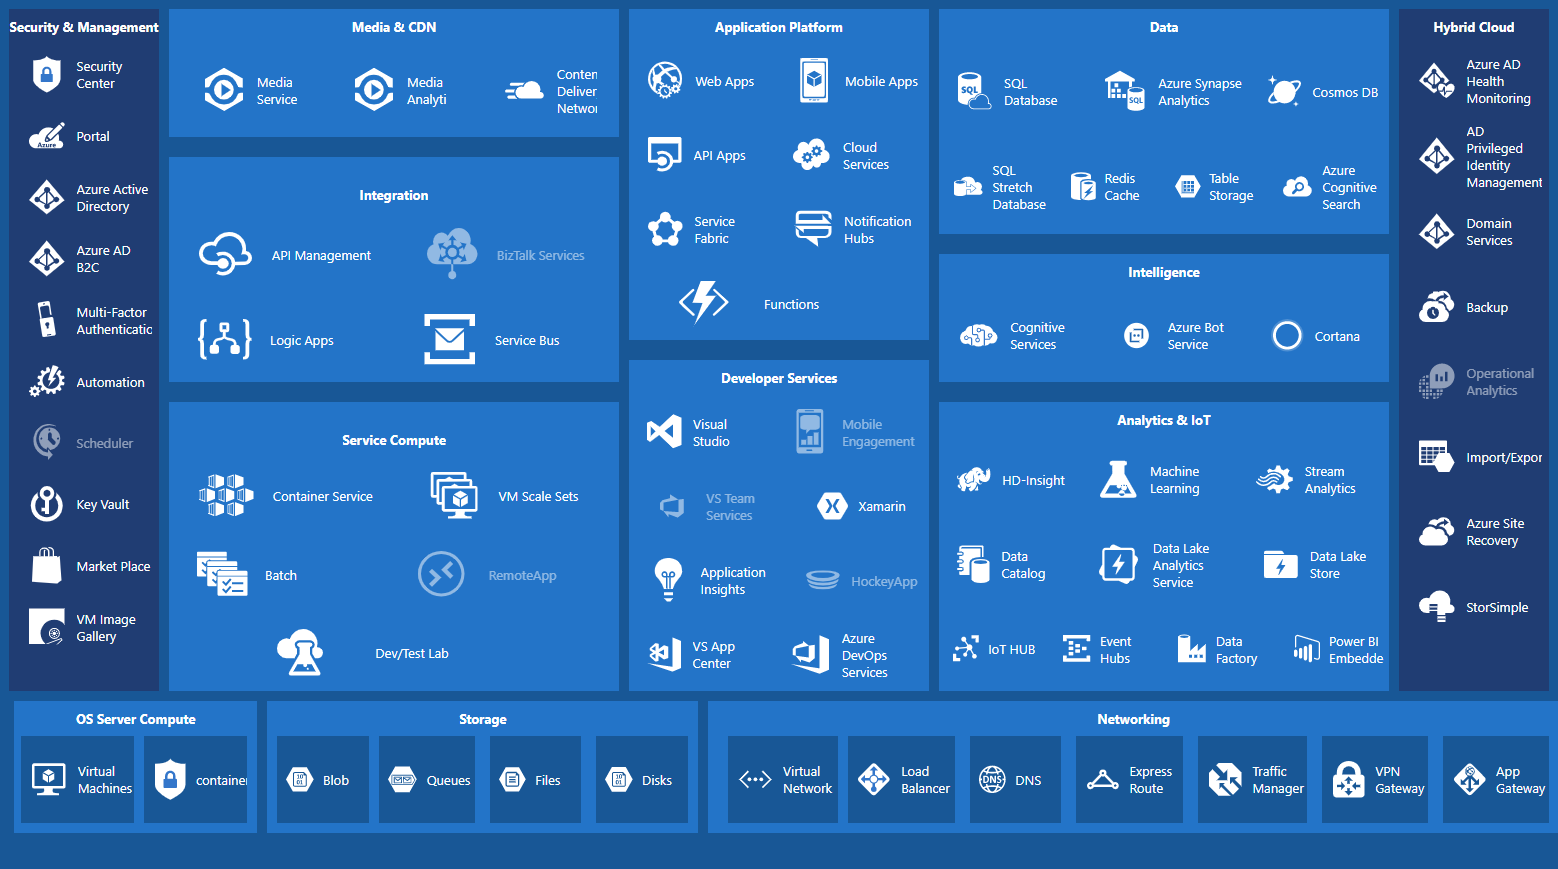
\includegraphics[width=\textwidth]{images/ms_azure}
    \captionsource{Schemat podziału usług MS Azure}{\cite{Datashifta}}
    \label{fig:ms-azure}
\end{figure}

\refsource{Schemat}{fig:ms-azure} pokazuje jak obecnie podzielone są usługi oraz co jest udostępnione komercyjnie w ramach platformy Azure.\ Według schematu platforma podzielona jest na trzynaście obszarów, do których zaliczono między innymi bezpieczeństwo, zarządzanie danymi, usługi deweloperskie, analiza danych, platformy aplikacji.

\section{Infrastruktura}
Infrastruktura globalna Azure składa się z dwóch części: fizycznej infrastruktury oraz globalnej łączności.\ Infrastruktura fizyczna składa się z ponad 200 centrów danych na całym świecie, połączonych w jedną globalną sieć.\ Takie rozwiązanie umożliwia wysoką skalowalność i dostępność poszczególnych rozwiązań.\ Cały ruch sieciowy jest utrzymywany wewnątrz prywatnej sieci Microsoft.\ Pozwala to na zachowanie informacje o adresach IP wewnątrz sieci, a co za tym idzie, informacje te nie trafiają do opinii publicznej~\cite{MicrosoftAzureb}.\\ \\

Na swojej stronie internetowej Microsoft udostępnia wirtualną mapę, umożliwiającą zobaczenie aktualnej sieci Microsoftu oraz jej rozmieszczenie na globie ziemskim.\ Interaktywna mapa pozwala uzyskiwać informację o poszczególnych krajach oraz centrach danych znajdujących się na terytoriach tych krajów.\ Mapę oraz informację pokazano na \refsource{zdjęciach}{fig:azure-ic}.

\vfill
\pagebreak

\begin{figure}[H]
    \begin{subfigure}[m]{0.7\textwidth}
    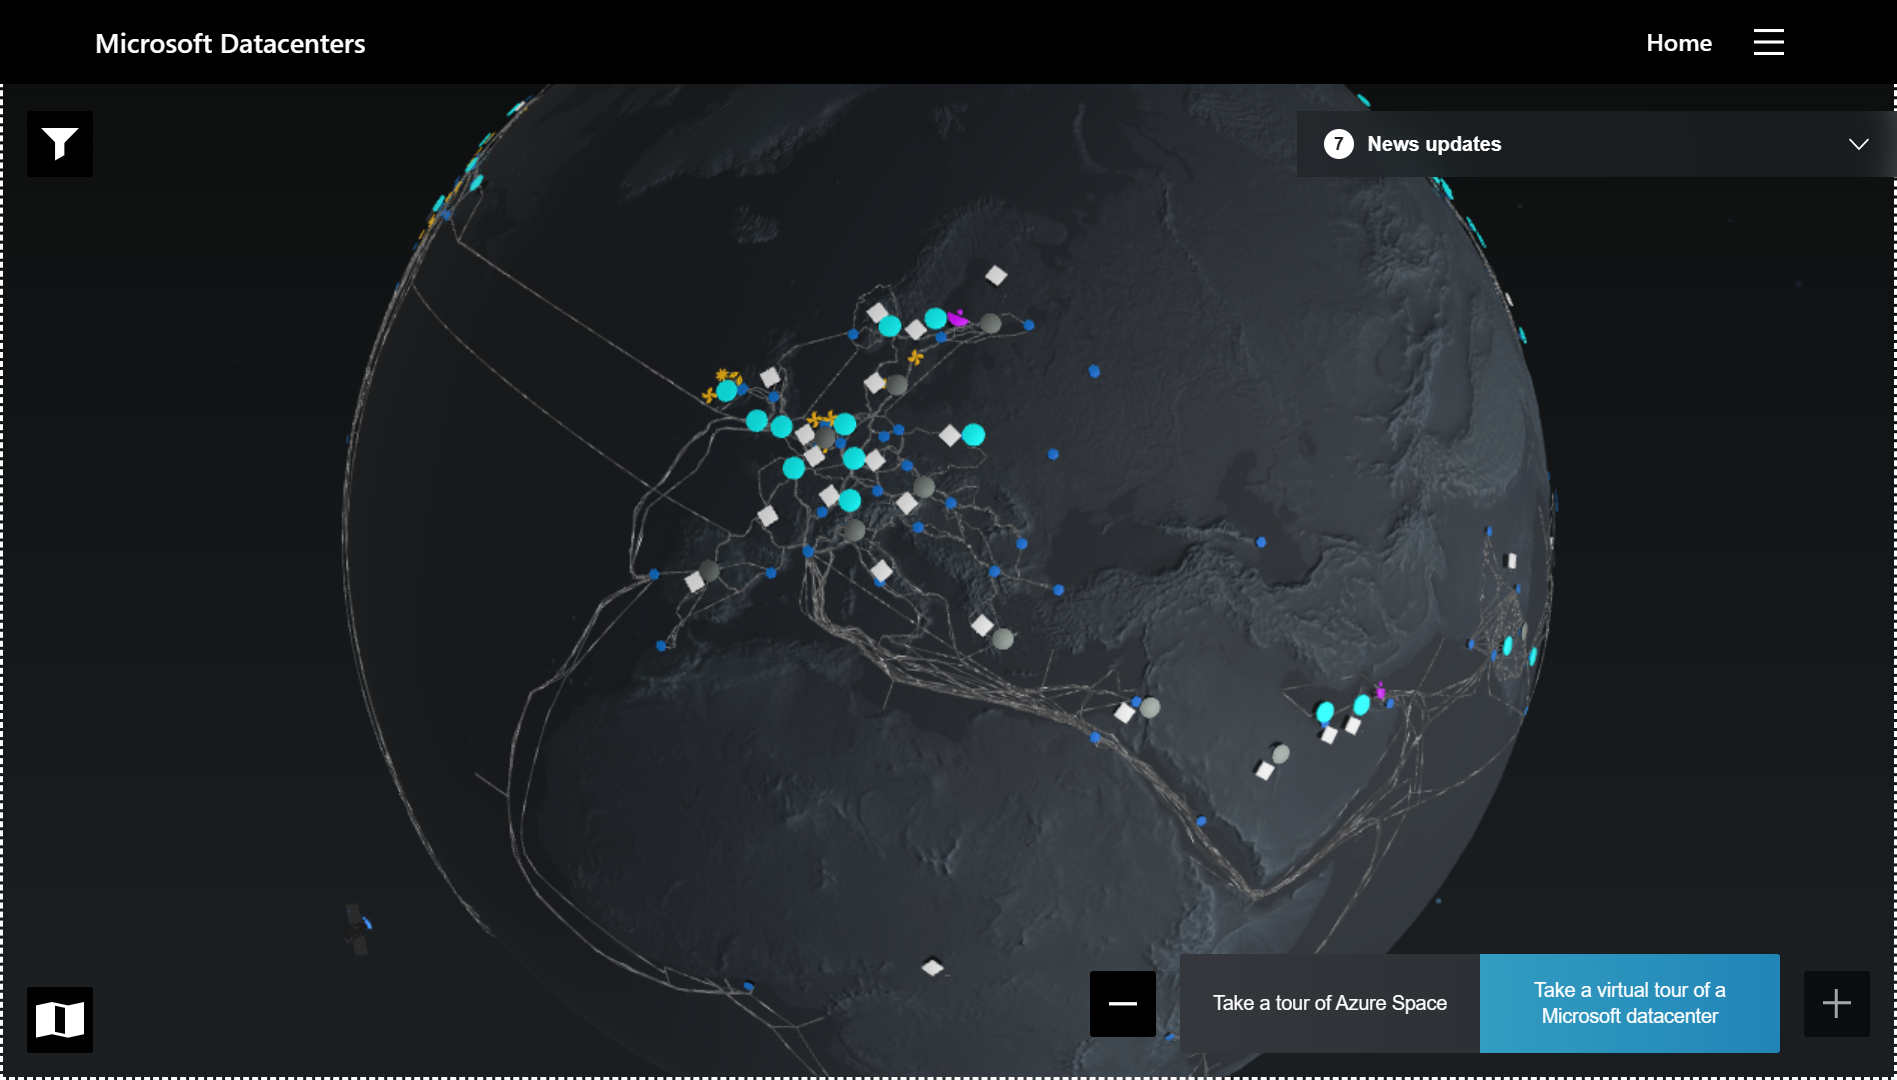
\includegraphics[width=\textwidth]{images/azure-ic}
    \captionsource{Globalna mapa infrastruktury sieciowe}{\cite{MicrosoftAzured}}
    \end{subfigure}
    \hfill
    \begin{subfigure}[m]{0.25\textwidth}
        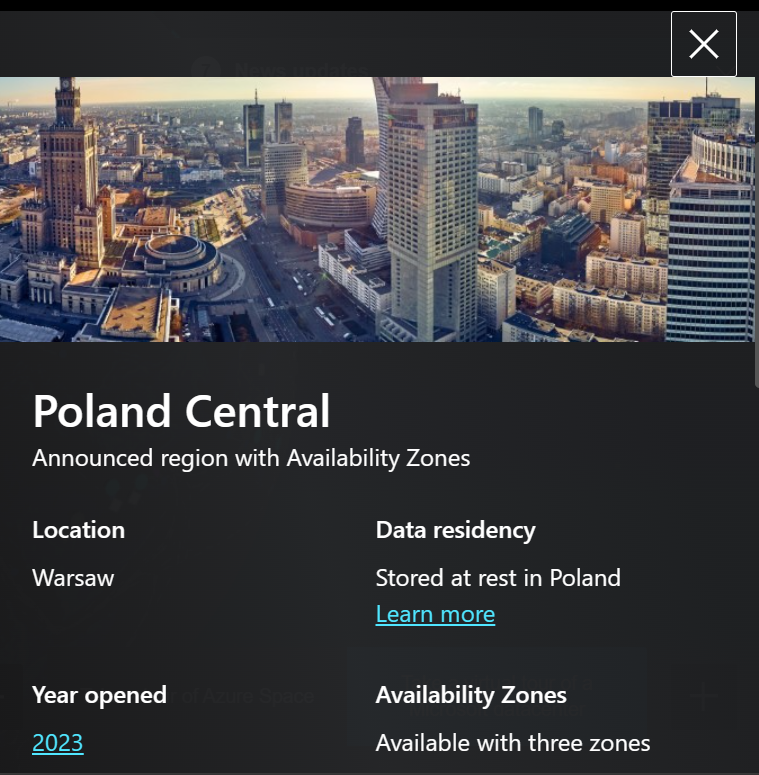
\includegraphics[width=\textwidth]{images/azure-pl}
        \captionsource{Informacje o centrum danych}{\cite{MicrosoftAzuree}}
    \end{subfigure}
    \captionsource{Zdjęcia z mapy insfrastruktury Microsoft Azure}{\cite{MicrosoftAzuree, MicrosoftAzured}}
    \label{fig:azure-ic}
\end{figure}

\section{Machine Learning Studio}
Azure Machine Learning Studio to platforma low-code.\ Umożliwia łatwe i szybkie tworzenie wysoce wydajnych modeli uczenia maszynowego, a także zarządzanie nimi.\ Użytkownik nie musi posiadać wiedzy teoretycznej związanej z uczeniem maszynowym czy programowaniem.\ Rozwiązanie wspiera pełen cykl życia kompleksowego uczenia maszynowego.\ Platforma umożliwia tworzenie potoków zadań, które połączone w jeden potok, wykonują poszczególne zadania w odpowiedniej kolejności.\ Mechanizm ,,\textit{złap i upuść}'' \textit{(ang. drag\&drop)} umożliwia tworzenie potoków w sposób graficzny.\ Dzięki modułowej budowie potoków można uzyskać rozwiązanie wielokrotnego użytku.\ W ramach jednego doświadczenia każdy moduł może byc buforowany.\ Pozwala to na ,,zapamiętanie'' wyniku poprzedniego uruchomienia i wykorzystanie go ponownie (o ile dane wejściowe albo konfiguracja nie uległy zmianie).\ Dodatkowo poza predefiniowanymi operacjami można wykorzystać moduły języka Python/R.\ Kolejną możliwością jest wytworzenie rozwiązania w technologii ,,\textbf{Jupiter Notebook}'' oraz wizualne narzędzie wykorzystujące mechanizm \textit{przeciągnij i upuść} \trans{ang. Drag \& Drop}.\ Rozwiązanie to pozwala układać ,,\textit{kafelki}'' służące do tworzenia potoków zadań.\ Każde zadanie wykorzystuje wcześniej przygotowaną jednostkę obliczeniową, dzięki czemu można przewidzieć albo dostosować koszt wykorzystania modelu.\ Umożliwione zostało również wdrażanie modeli jako punktów końcowych.\ Pozwala to na komunikowanie się z nimi za pomocą REST API.
\\ \\
Microsoft umożliwia płatność jedynie za użytkowanie usług, co oznacza, że jeśli klaster komputerowy był wykorzystywany jedynie przez 1 godzinę, to za tą jedną godzinę zostanie obciążony klient\cite{MicrosoftAzuref}.
	\chapter{Opis doświadczenia}
\label{cha:dos}
Przeprowadzone doświadczenie polega na porównaniu dostępnych w środowisku Microsoft Azure algorytmów klasyfikacji danych dwuklasowych wraz z algorytmem stworzonym na potrzeby pracy inżynierskiej o tytule ,,\textit{Wykorzystanie algorytmów genetycznych w systemach wykrywania intruzów w sieciach komputerowych}''~\cite{Blyszcz2022} oraz z algorytmem DANet~\cite{Chen2022}.\ Doświadczenie przebiegało według \refsource{schematu}{fig:sch-prac}.

\begin{figure}[H]
    \centering
    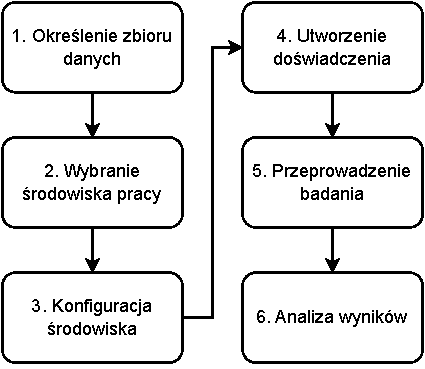
\includegraphics[width=0.9\textwidth]{images/schemat_pracy}
    \captionsource{Schemat przebiegu doświadczenia}{Opracowanie własne}
    \label{fig:sch-prac}
\end{figure}

\vfill
\pagebreak

\section{Założenie techniczne}

Dane prezentowane w \refsource{Tabeli}{tab:technical} określają podstawowe założenia techniczne przyjęte w trakcie wykonywania analizy porównawczej.\ Dane te dotyczą między innymi środowiska, w którym wykonane było doświadczenie.\ Dodatkowo uwzględniono zestaw danych oraz biblioteki użyte w trakcie tworzenia doświadczenia.

\begin{table}[H]
    \centering
    \captionsource{Założenia techniczne pracy dyplomowej}{Opracowanie własne}
    \label{tab:technical}
    \begin{tabular}{|l|l|}
        \hline
        \textbf{Środowisko uruchomieniowe} & Machine Learning Studio\cite{azureml} \\ \hline
        \textbf{Język programowania} & Python 3.x \\ \hline
        \multirow{3}*{\textbf{Wykorzystane biblioteki}} & scikit-learn~\cite{scikit-learn} \\
        \cline{2-2}
        & Numpy~\cite{Harris2019} \\
        \cline{2-2}
        & Pandas~\cite{pandas, McKinney2010} \\
        \hline
        \textbf{Wykorzystane dane} & CICDS2017~\cite{cicds2017kaggle} \\
        \hline
    \end{tabular}
\end{table}

\section{Dane}
\label{sec:data}
Zbiór danych został przygotowany przez Kanadyjski Instytut Cyberbezpieczeństwa działający przy Uniwersytecie Nowy Brunszwik.\ Został wykonany za pomocą narzędzia CICFlowMeter
~\cite{Ahlashkari2022}.\ Zbiór zawiera 79 cech ruchu sieciowego, do których zaliczyć można:
\begin{enumerate}
    \item etykietę,
    \item czas trwania przesyłu,
    \item minimalną długość pakietu zwrotnego,
    \item maksymalną długość pakietu zwrotnego,
    \item port docelowy,
    \item długość pakietów.
\end{enumerate}
Zbiór pozwala na określenie czy ruch sieciowy jest życzliwy \trans{ang. BENING}, czy nieżyczliwy (różne możliwe formy ataku na sieć).\ Dodatkowo zbiór został podzielony na pięć dni roboczych: poniedziałek 3.07.2017 - piątek 7.07.2017.\ Dane z poniedziałku zawierają jedynie ruch życzliwy.\ W pozostałe dni zostały zasymulowane ataki na sieć komputerową~\cite{Blyszcz2022, unbkaggle}.

\section{Programistyczne środowisko badawcze}
Jako środowisko programistyczne zostało wybrane Azure Machine Learning Studio.\ Zostało to spowodowane możliwością uniezależnienia obliczeń od komputera lokalnego.\ Platforma umożliwia łatwy sposób na tworzenie skomplikowanych potoków zadań, które składają się z komponentów wielokrotnego użytku.\ Każdy komponent uruchamia się w środowisku odizolowanym od pozostałych operacji.\ Dzieje się tak dzięki wykorzystaniu wielowęzłowych klastrów obliczeniowych, bazujących na oprogramowaniu Docker.\ Klastry te mogą skalować się w zależności od potrzeb oraz dostępnej jednostki~\cite{MicrosoftLearn2023}.
\\ \\
Całe doświadczenie zostało odwzorowane w graficznym potoku narzędzia ,,\textit{Projektant}'' oraz przedstawione na \refsource{zdjęciu}{fig:pipeline}.

\begin{landscape}
    \centering
\begin{figure}[H]
    \centering
    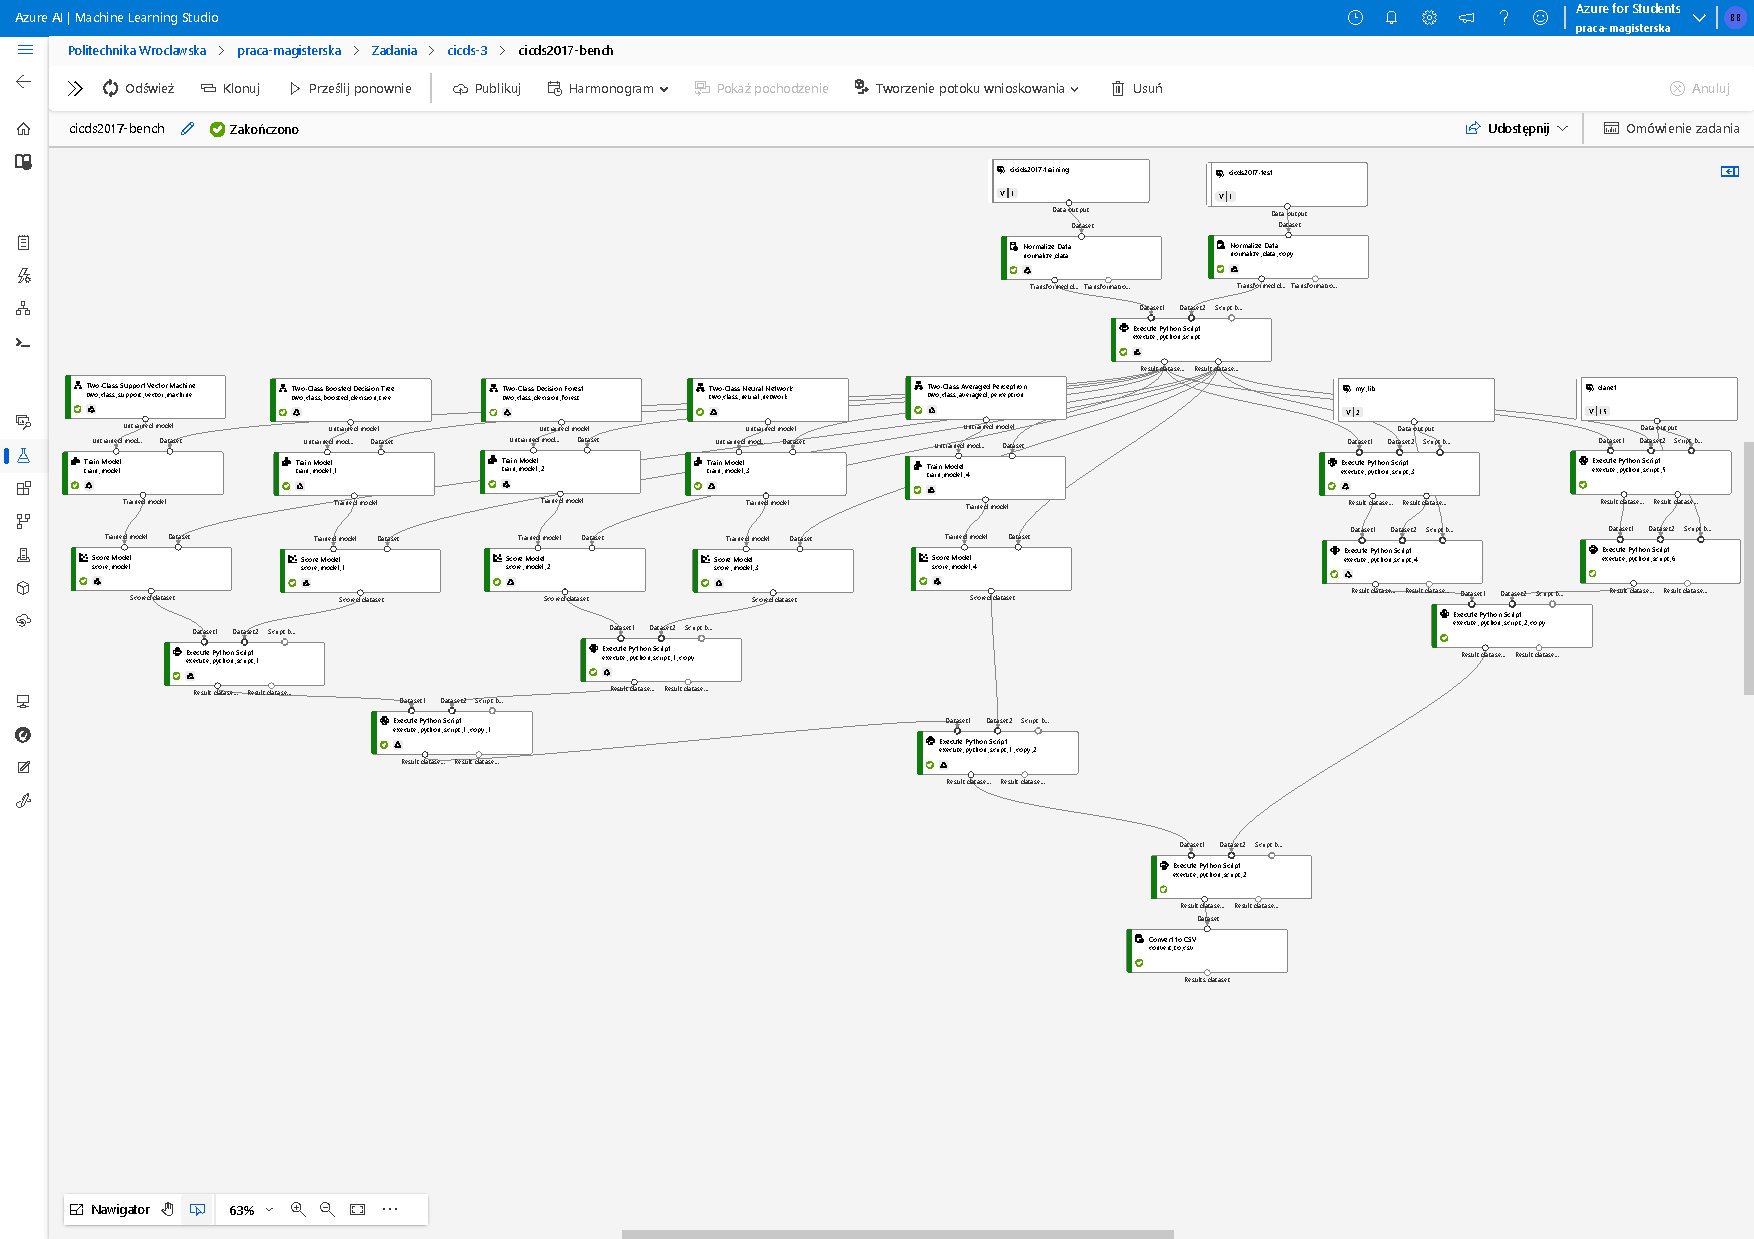
\includegraphics[height=0.9\textwidth]{images/pipeline}
    \captionsource{Potok zadań}{Opracowanie własne}
    \label{fig:pipeline}
\end{figure}
\end{landscape}

\section{Algorytmy}
\label{sec:alg}
W trakcie eksperymenty zastosowano różne algorytmy klasyfikacji danych.\ Charakterystyczną cechą tych algorytmów jest klasyfikacja ukierunkowana na 2 kategorie wejściowe.\ W tym wypadku są to kategorie ruchu sieciowego: [\textbf{BENIGN} \trans{pl. życzliwy}, \textbf{OTHER} \trans{pl. inne}], gdzie inne to pozostałe typy ruchu sieciowego.

\subsection{Two-Class Support Vector Machine}
Algorytm SVM ma za zadanie znaleźć hiperpłaszczyznę w przestrzeni K-wymiarowej (K - liczba cech), która rozdziela zbiory punktów odpowiadających różnym klasom.\ W pierwszej kolejności szuka się separatora między klasami, a następnie przekształca się dane w taki sposób, by można przekształcić separator w hiperpłaszczyznę~\cite{IBM}.\ Sposób działania został zobrazowany za pomocą \refsource{wykresów}{fig:svm-schem}.\ Część \refsource{potoku}{fig:pipeline} odpowiedzialnego za SVM to \refsource{schemat}{fig:svm-pipe}.

\begin{figure}[H]
    \begin{subfigure}[m]{0.45\textwidth}
        \centering
        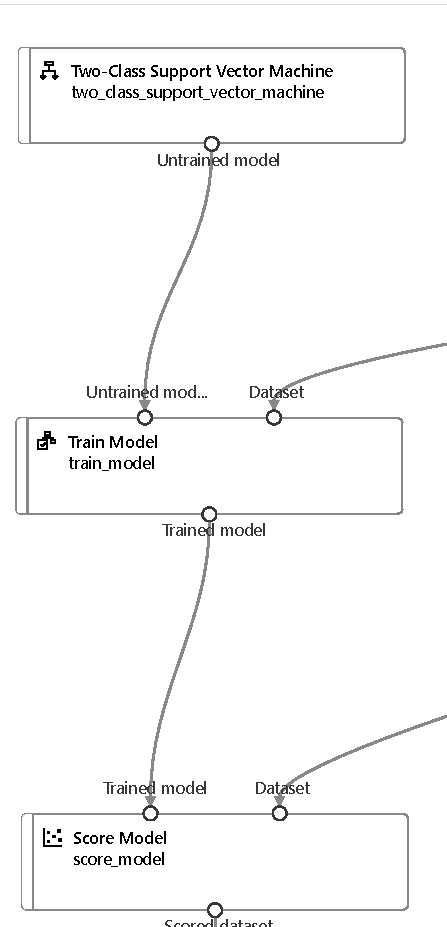
\includegraphics[width=\textwidth]{images/svm_pipe}
        \captionsource{Potok zadań dla modelu \textit{Two-Class Support Vector Machine}}{Opracowanie własne}
        \label{fig:svm-pipe}
    \end{subfigure}
    \hfill
    \begin{subfigure}[m]{0.45\textwidth}
        \centering
        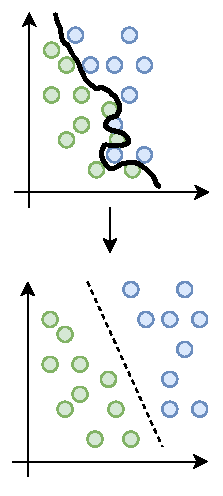
\includegraphics[width=\textwidth]{images/svm}
        \captionsource{Schemat SVM}{\cite{Statsoft}}
        \label{fig:svm-schem}
    \end{subfigure}
\end{figure}

\vfill
\pagebreak

\subsection{Two-Class Boosted Decision Tree}
Jest to algorytm drzewa decyzyjnego oparty o algorytm LightGBM.\ Dzięki zastosowaniu tego podejścia algorytm oparty o drzewo decyzyjne działa szybciej oraz ma mniejszą złożoność obliczeniową.\ Algorytm ten działa na zasadzie doboru odpowiedniego liścia, zamiast jak w przypadku klasycznych algorytmów opartych na drzewie, wyboru odpowiedniej warstwy~\cite{LightGBM}.\ Sposób podejścia liściastego został ukazany na \refsource{schemacie}{fig:leaf}.\ Model wykorzystywany w Azure ML został ukazany na \refsource{rysunku}{fig:dt-pipe}.
\begin{figure}[H]
    \begin{subfigure}[m]{0.3\textwidth}
        \centering
        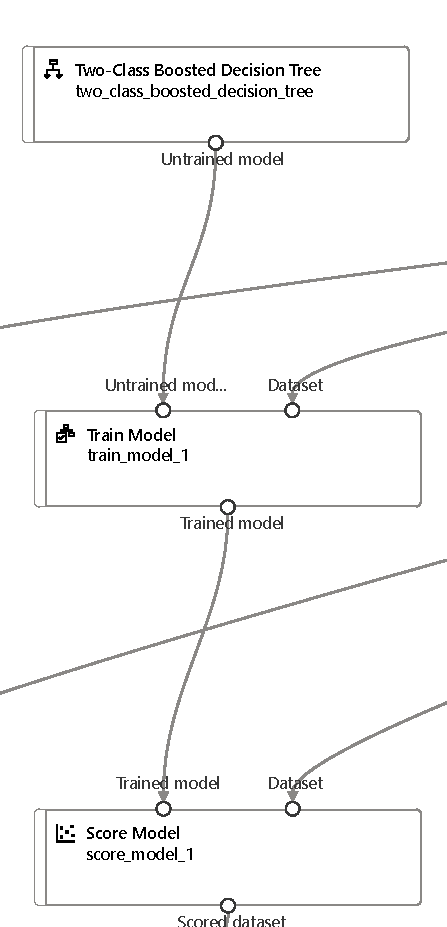
\includegraphics[width=\textwidth]{images/dt_pipe}
        \captionsource{Potok zadań dla modelu \textit{Two-Class Boosted Decision Tree}}{Opracowanie własne}
        \label{fig:dt-pipe}
    \end{subfigure}
    \hfill
    \begin{subfigure}[m]{0.66\textwidth}
        \begin{subfigure}[m]{\textwidth}
            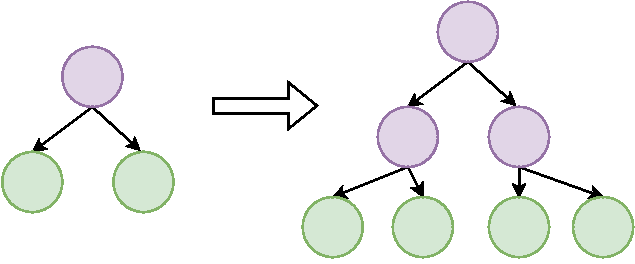
\includegraphics[width=\textwidth]{images/level-wise}
        \end{subfigure}
        \begin{subfigure}[m]{\textwidth}
            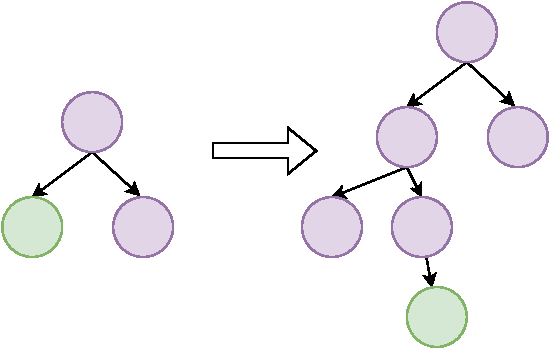
\includegraphics[width=\textwidth]{images/leaf-wise}
        \end{subfigure}
        \captionsource{Sposób działania algorytmu}{\cite{LightGBM}}
        \label{fig:leaf}
    \end{subfigure}
\end{figure}
\vfill
\pagebreak

\subsection{Two-Class Decision Forest}
Las decyzyjny to algorytm, którego wynik opiera się o agregację wyników wielu drzew decyzyjnych.\ Uzyskanie wyniku zależy od algorytmu trenowania lasu.\ Przykładowo w klasyfikacji losowym lasem wieloklasowym \trans{ang. Multi-class random forest classification}, każde drzewo głosuje na jedną klasę.\ Klasa, która zostanie wybrana większością głosów, zostaje uznana za wynikową~\cite{Google}.\ Model wykorzystany w Azure ML pokazano na \refsource{modelu}{fig:df-pipe}

\begin{figure}[H]
    \centering
    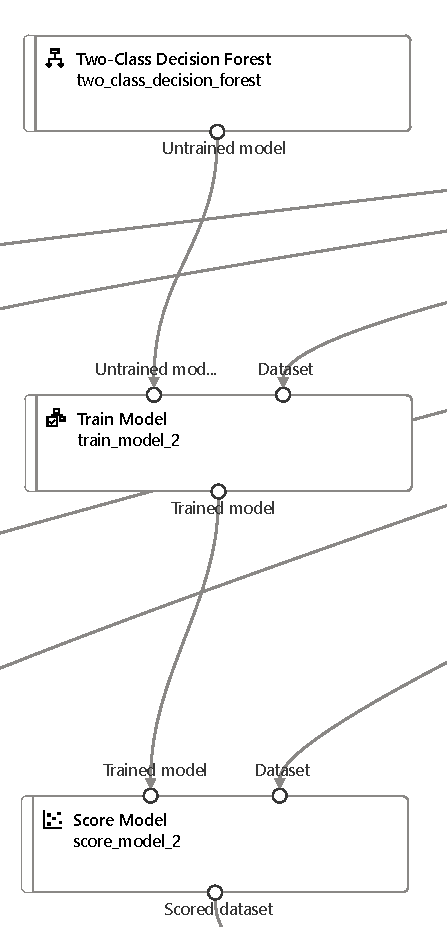
\includegraphics[width=0.3\textwidth]{images/df_pipe}
    \captionsource{Potok zadań dla modelu \textit{Two-Class Decision Forest}}{Opracowanie własne}
    \label{fig:df-pipe}
\end{figure}

\vfill
\pagebreak

\subsection{Two-class Neural Network}
Jest to sieć neuronowa, która składa się z warstwy wejściowej, trzech warstw ukrytych (każda posiada po 100 węzłów), oraz z warstwy wyjściowej.\ Przykładowa sieć neuronowa została zobrazowana na \refsource{schemacie}{fig:neural-network}.\ Moduł wykorzystany w Azure ML ukazano na \refsource{rysunku}{fig:nn-pipe}.

\begin{figure}[H]
    \centering
    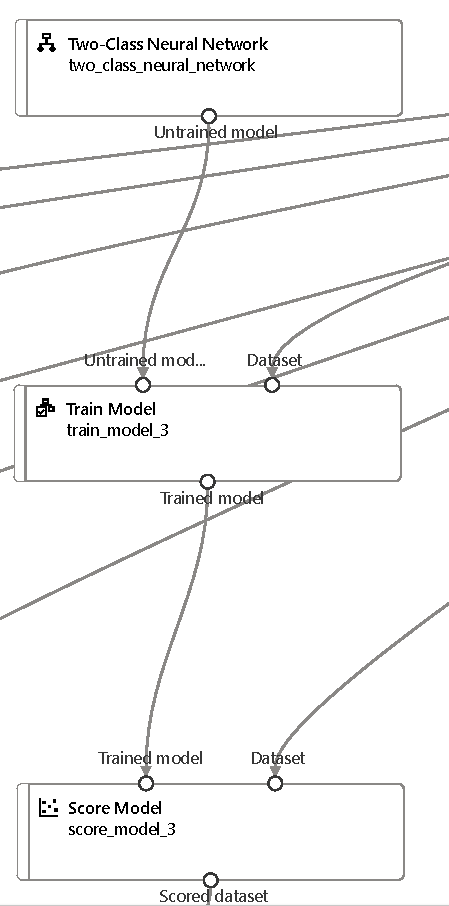
\includegraphics[width=0.3\textwidth]{images/nn_pipe}
    \captionsource{Potok zadań dla modelu \textit{Two-Class Neural Network}}{Opracowanie własne}
    \label{fig:nn-pipe}
\end{figure}

\vfill
\pagebreak

\subsection{Two-Class Average Perceptron}
Jest to najprostsza odmiana sieci neuronowej, czyli pojedynczy perceptron, który jest matematycznym modelem neuronu.\ Składa się on z \textit{n} wejść, takiej samej ilości wag, progu $\Theta$, sumatora, funkcji aktywującej i wyjścia.\ Został zobrazowany na \refsource{schemacie}{fig:neuron}.\ Może służyć za prosty klasyfikator binarny albo za regresor.\ Model wykorzystany w Azure ML ukazano na \refsource{zdjęciu}{fig:ap-pipe}.

\begin{figure}[H]
    \centering
    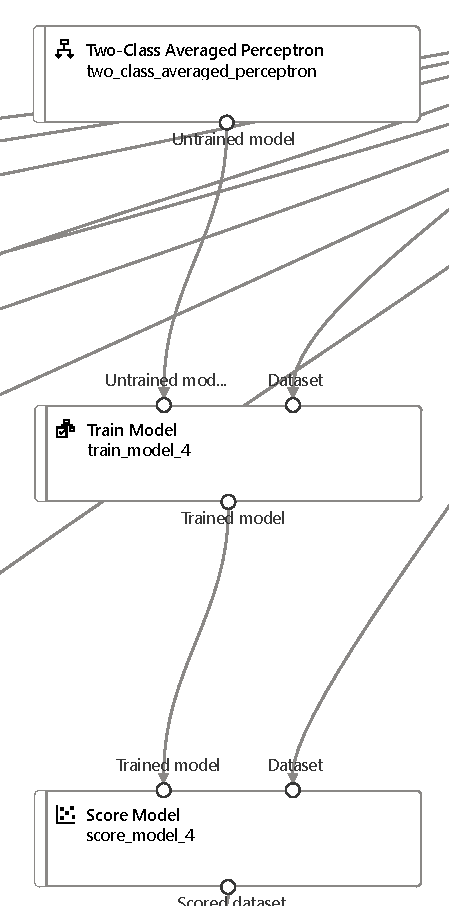
\includegraphics[width=0.3\textwidth]{images/ap_pipe}
    \captionsource{Potok zadań dla modelu \textit{Two-Class Average Perceptron}}{Opracowanie własne}
    \label{fig:ap-pipe}
\end{figure}

\vfill
\pagebreak

\subsection{Gausian Naive Bayes - with GA}
Algorytm ten polega na połączeniu algorytmu genetycznego (GA) wraz z klasyfikatorem naiwnym Bayesa wykorzystującego rozkład Gaussa (GNB).\ Zadaniem algorytmu genetycznego jest znalezienie najistotniejszych cech w zbiorze tabelarycznym.\ Poszukiwane cechy powinny pozwolić na zmniejszenie wymiarowości danych oraz na zmniejszenie kosztów obsługi samego klasyfikatora.\ Co może zostać uzyskane późniejszych etapach testowania, ze względu na zmniejszoną ilość danych wymaganych do przetworzenia.\ GA wykorzystywał w metodzie \textbf{fitness} algorytm GNB w celu określenia dopasowania danych.\ Zadaniem GNB było znalezienie najlepszej dostępnej kombinacji cech, które pozwalały na uzyskanie najlepszego dopasowania~\cite{Blyszcz2022}.\ Model wykorzystywany w Azure ML różni się od gotowych modeli tym, że dołączono do niego bibliotekę napisaną w języku Python, która zawiera kod wykorzystywany w pracy inżynierskiej autora~\cite{Suvres2023}.
\begin{figure}[H]
    \centering
    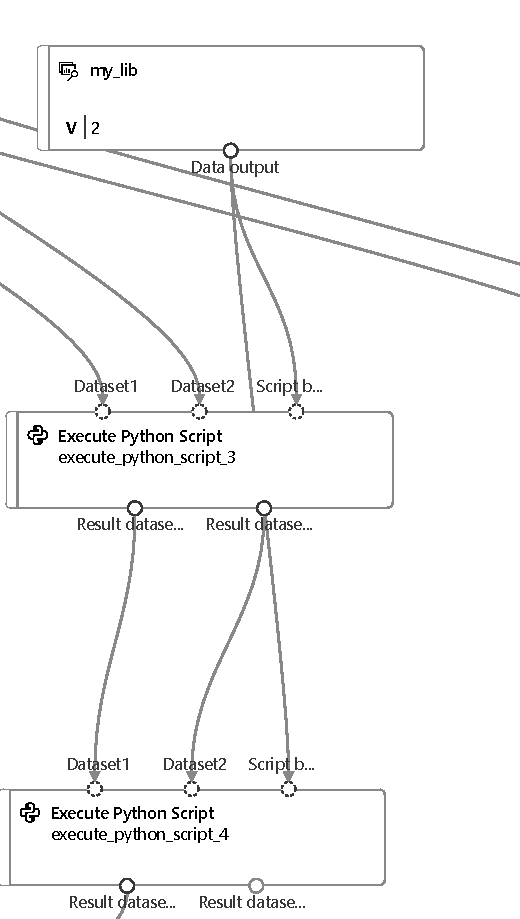
\includegraphics[width=0.3\textwidth]{images/ga_pipe}
    \captionsource{Potok zadań dla modelu}{Opracowanie własne}
    \label{fig:ga-pipe}
\end{figure}

\vfill
\pagebreak

\subsection{DANet}
Twórcy tego algorytmu wprowadzają dodatkową warstwę abstrakcyjną o nazwie ,,\textit{Abstract Layer}''.\ Warstwy te budują sieć o nazwie ,,\textit{Deep Abstract Network}'' (DANet).\ Zadanie dodatkowych warstw jest grupowanie cech w skorelowanych zbiorach.\ Zbiory te budują sieć powiązań między sobą w formie sieci semantycznej.\ Gdy sieć semantyczna jest zbudowana, to w ostatnim kroku wykonywana jest klasyfikacja w trzywarstwowej sieci perceptronów \trans{ang. Multilayer Perceptron network} (MLP)~\cite{Chen2022, Danet}.\ Model znajdujący się z Azure ML został przedstawiony na \refsource{zdjęciu}{fig:danet-pipe}, zaś sposób działania ukazano na \refsource{schematach}{fig:danet-abst}.

\begin{figure}[H]
    \begin{subfigure}[m]{0.49\textwidth}
        \centering
        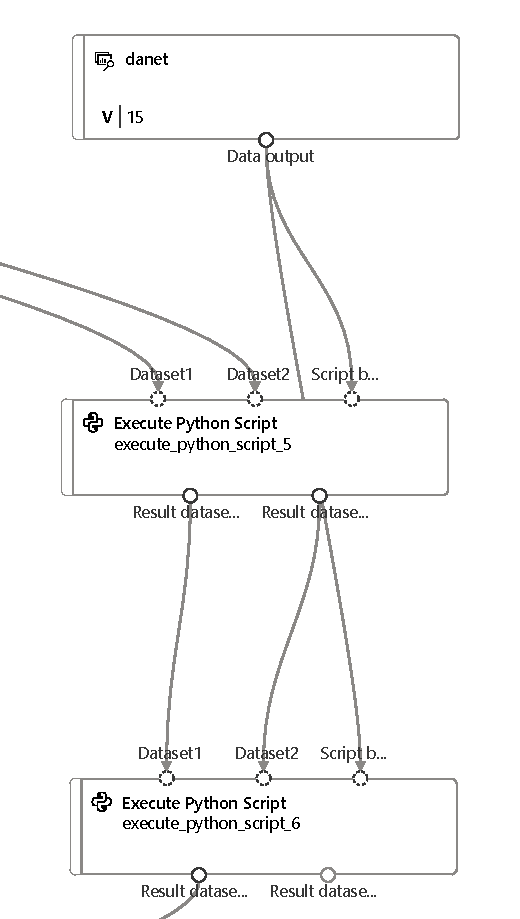
\includegraphics[width=0.4\textwidth]{images/danet}
        \captionsource{Potok zadań dla modelu \textit{DANet}}{Opracowanie własne}
        \label{fig:danet-pipe}
    \end{subfigure}
    \hfill
    \begin{subfigure}[m]{0.49\textwidth}
        \begin{subfigure}[m]{\textwidth}
            \centering
            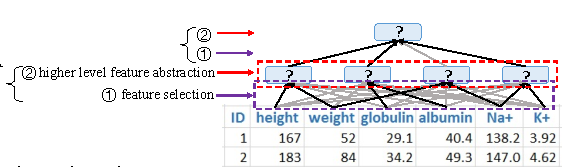
\includegraphics[width=\textwidth]{images/danet_1}
        \end{subfigure}
        \begin{subfigure}[m]{\textwidth}
            \centering
            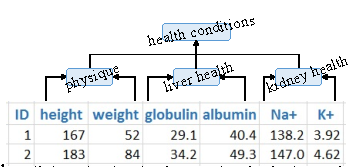
\includegraphics[width=\textwidth]{images/danet_2}
        \end{subfigure}
        \captionsource{Sposób działania DANet}{\cite{Chen2022}}
        \label{fig:danet-abst}
    \end{subfigure}

\end{figure}





	\chapter{Przebieg badań}
Doświadczenie polegało na analizie porównawczej sprawności algorytmów opisanych w \refsource{rozdziale}{cha:dos} w \refsource{sekcji}{sec:alg}. Celem doświadczenia było określenie jakości algorytmu utworzonego w ramach pracy inżynierskiej autora\cite{Blyszcz2022}. Szczegółowa metodologia badawcza została określona w \refsource{podrozdziale}{sec:met}.

\section{Metodologia badawcza}
\label{sec:met}
Przyjęta w projekcie metodologia badawcza została określona w poniższej \refsource{tabeli}{tab:met-bad}. Przyjęta metodologia ma za zadanie określić jakoś porównywanego algorytmu.

\begin{table}[H]
    \centering
    \captionsource{Metodologia badawcza}{Opracowanie własne}
    \begin{tabular}{|L{\textwidth}|}
        \hline
        \textbf{Problem badawczy:} \\
        Czy algorytm klasyfikacji danych utworzony w ramach pracy inżynierskiej może konkurować z rozwiązaniami dostępnymi w środowiskach komercyjnych \\ \hline

        \textbf{Pytania badawcze:} \\
        \begin{enumerate}
            \item Czy algorytm jest konkurencyjny pod względem wybranych metry:
            \begin{itemize}
                \item dokładność algorytmu
                \item czas działania
                \item precyzja
                \item czułość
                \item f1
                \item auc
            \end{itemize}
        \end{enumerate} \\ \hline

        \textbf{Hipotezy:} \\
        \begin{enumerate}
            \item Nie ma istotnej różnicy w uzyskanej ''\textit{dokładności}'' między algorytmami.
            \item Nie ma istotnej różnicy w uzyskanej ''\textit{czułości}'' między algorytmami.
            \item Nie ma istotnej różnicy w uzyskanej ''\textit{precyzji}'' między algorytmami.
            \item Nie ma istotnej różnicy w uzyskanym ''\textit{auc}'' między algorytmami.
            \item Nie ma istotnej różnicy w uzyskanej ''\textit{f1}'' między algorytmami.
            \item Nie ma istotnej różnicy w uzyskanym ''\textit{czasie działania}'' między algorytmami.
        \end{enumerate} \\ \hline
    \end{tabular}
    \label{tab:met-bad}
\end{table}

\section{Przygotowanie platformy}
Do badań wykorzystano narzędzie ''\textit{Projektant}'' znajdujące się na platformie ''\textit{Azure Machine Learning Studio}'' (Azure ML). Narzędzie to umożliwiło utworzenie interaktywnego potoku zadań. Potok ten składa się z kilku części:
\begin{itemize}
    \item Przygotowanie i obróbka zbiorów danych
    \item Trenowanie oraz testowanie algorytmów klasyfikacji danych
    \item Utworzenie tabeli porównawczej dla wyników poszczególnych algorytmów (\refsource{obraz}{fig:pipeline}).
\end{itemize}

\subsection{Przygotowanie danych}
W pierwszym kroku dane zostały znormalizowane za pomocą metody \textbf{MinMax}, która przekształca dane numeryczne do wartości w zakresie ${0, 1}$. W następnym kroku za pomocą języka Python oraz biblioteką Pandas oraz Numpy zostają zamienione etykiety słowne na wartości \textbf{0} i \textbf{1} oraz następuje zamiana wartości $[NaN, -inf, inf]$ na cyfrę $0$. Cały proces został zobrazowany na \refsource{diagramie}{fig:norm}

\begin{figure}[H]
    \centering
    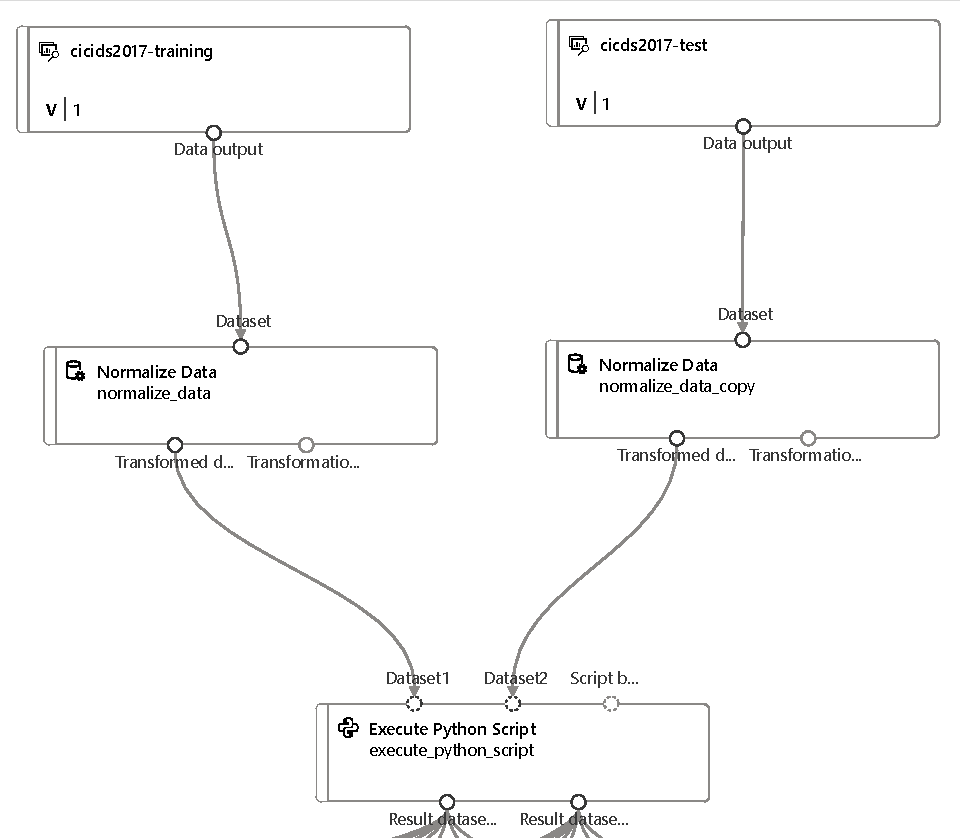
\includegraphics[width=0.6\textwidth]{images/norm}
    \captionsource{Potok normalizacji danych}{Opracowanie własne}
    \label{fig:norm}
\end{figure}

\subsection{Trenowanie oraz testowanie algorytmów}
Kolejną grupą zadań widoczną w potoku są te związane z trenowaniem i testowaniem poszczególnych algorytmów opisanych w \refsource{rozdziale}{cha:dos}. Każdy test składa się 3 kafelek. W przypadku algorytmów dostarczonych wraz z platformą Azure ML są to:
\begin{itemize}
    \item \textbf{model klasyfikujący} - odpowiada za przygotowanie algorytmu klasyfikacyjnego
    \item \textbf{blok treningowy} - tworzy wytrenowany model, za pomocą połączonego zbioru danych
    \item \textbf{blok ewaluacyjny} - sprawdza wcześniej wytrenowany model za pomocą powiązanego zbioru danych.
\end{itemize}
Potok zadań wykorzystujący algorytmy dostarczone przez Microsoft Azure został ukazany na \refsource{schemacie}{fig:ms-pipe}

\begin{figure}[H]
    \centering
    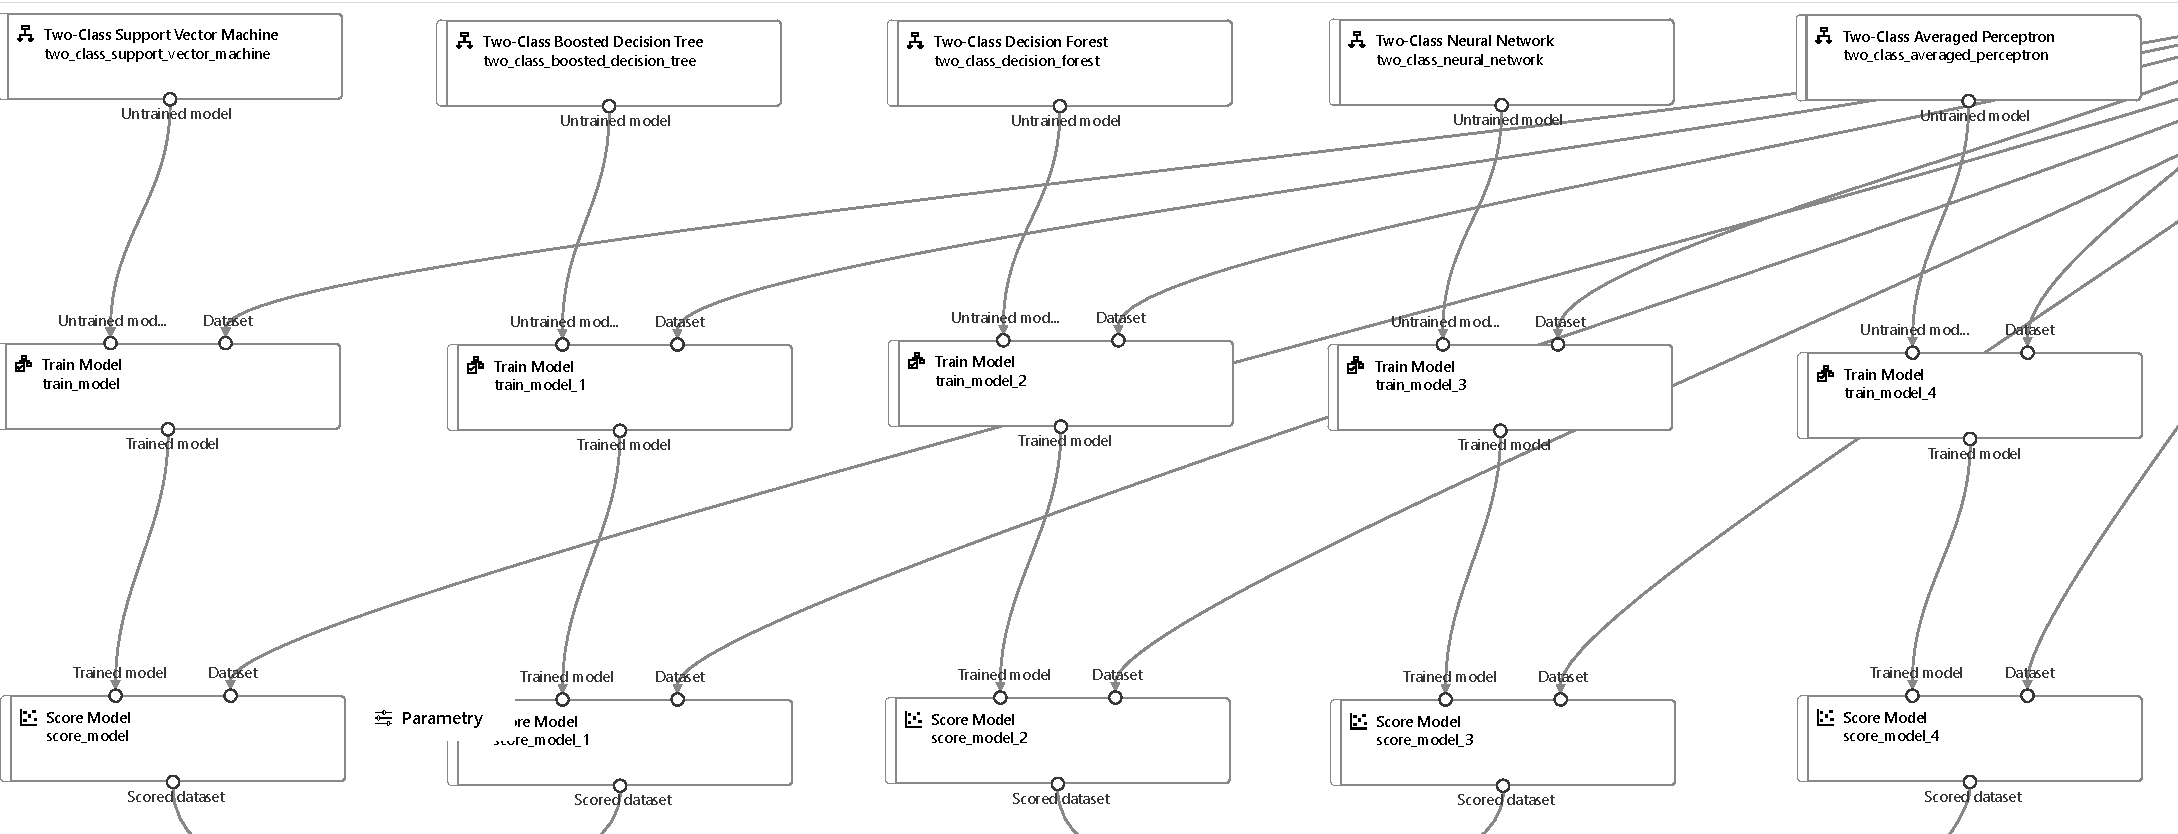
\includegraphics[width=\textwidth]{images/ms_pipe}
    \captionsource{Potok zadań dla algorytmów klasyfikacyjnych}{Opracowanie własne}
    \label{fig:ms-pipe}
\end{figure}

Algorytmy dostarczone w ramach pracy badawczej składają się z:
\begin{itemize}
    \item \textbf{biblioteka Python} - archiwum o rozszerzeniu \textbf{.zip}, które zawiera w sobie odpowiednie pliki napisane w języku Python
    \item \textbf{blok treningowy} - wykorzystuje dostarczoną bibliotekę do wytrenowania modelu oraz zapisania na platformie Azure najlepszego uzyskanego wyniku za pomocą powiązanego zbioru danych
    \item \textbf{blok ewaluacyjny} - wykorzystuje dostarczoną bibliotekę do ewaluacji algorytmu za pomocą połączonego zbioru danych
\end{itemize}

Potok zadań dla algorytmów niestandardowych został ukazany na \refsource{rysunku}{fig:au-pipe}

\begin{figure}[H]
    \centering
    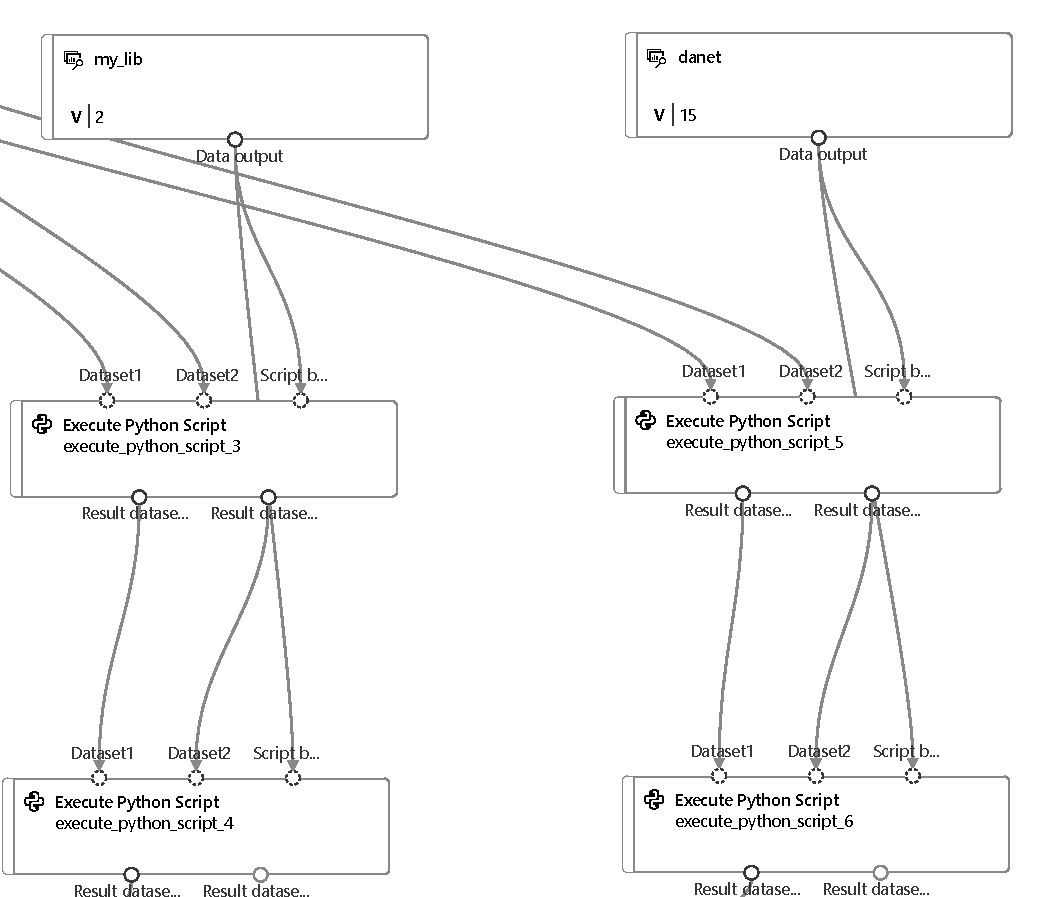
\includegraphics[width=0.8\textwidth]{images/au-pipe}
    \captionsource{Potok zadań dla algorytmów klasyfikacyjnych}{Opracowanie własne}
    \label{fig:au-pipe}
\end{figure}


\subsection{Utworzenie tabeli porównawczej}
Kolejną częścią zadań jest zebranie wyników poszczególnych algorytmów oraz połączenie ich w jedną całość. Wykorzystano do tego moduły języka Pyton, które zwracają przetwożone wyniki oraz łączą je w jedną tabelę zbiorczą, co pokazano na \refsource{rysunku}{fig:pipe-4}.

\begin{figure}[H]
    \centering
    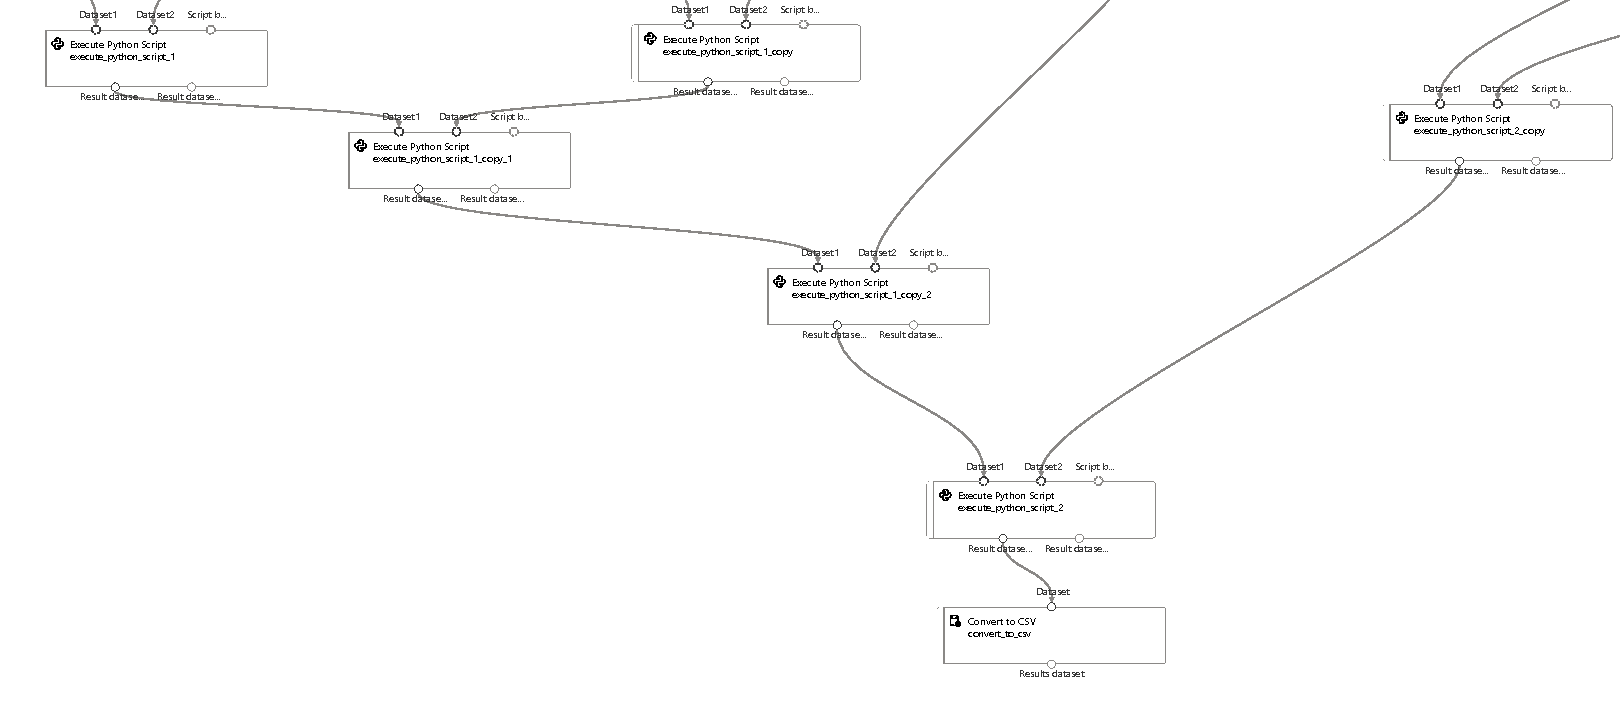
\includegraphics[width=\textwidth]{images/pipe-csv}
    \captionsource{Moduły odpowiedzialne za przetwożenie wyników}{Opracowanie własne}
    \label{fig:pipe-4}
\end{figure}

\section{Weryfikacja potoku}
Aby zweryfikować działanie całego procesu wykorzystano znormalizowane dane treningowe do wytrenowania oraz przetestowania działania algorytmów klasyfikacyjnych. Cały proces trwał ''\textbf{1 dzień 10 godzin 55 minut 53 sekundy}''. Wyniki tych działań widać na \refsource{rysunku}{fig:predict-same}. Analizując wykres można zauważyć, że uzyskane wyniki znajdują się w przedziale $[94\%, 100\%]$ w każdej metryce co pokazuje jakość każdego z algorytmów, a także to, że algorytmy poradziły sobie niemal bezbłędnie w rozpoznawaniu ruchu sieciowego, na którym były uczone. Zbiór, który wykorzystano do trenowania oraz testowania danych zawierał w sobie 225805 wpisów z czego 97718 należało do klasy ''\textbf{1}'', zaś 128087 należało do klasy ''\textbf{0}''.

\begin{table}[H]
    \centering
    \captionsource{Liczba elementów przynależących do danej klasy w zniorze treningowym}{Opracowanie własne}
    \label{tab:trening-data-label}
    \begin{tabular}{|c|r|} \hline
        \textbf{Klasa} & \textbf{Liczba wystąpień} \\ \hline
        1 & 97718 \\ \hline
        0 & 128027 \\ \hline
        \textbf{Suma} & 225805 \\ \hline
    \end{tabular}
\end{table}

Bazując na tym zbiorze oraz uzyskanych wynikach udało się udowodnić poprawność działania procesu klasyfikacji wieloma algorytmami genetycznymi.

\begin{landscape}
    \vspace*{\fill}
    \begin{figure}[H]
        \centering
        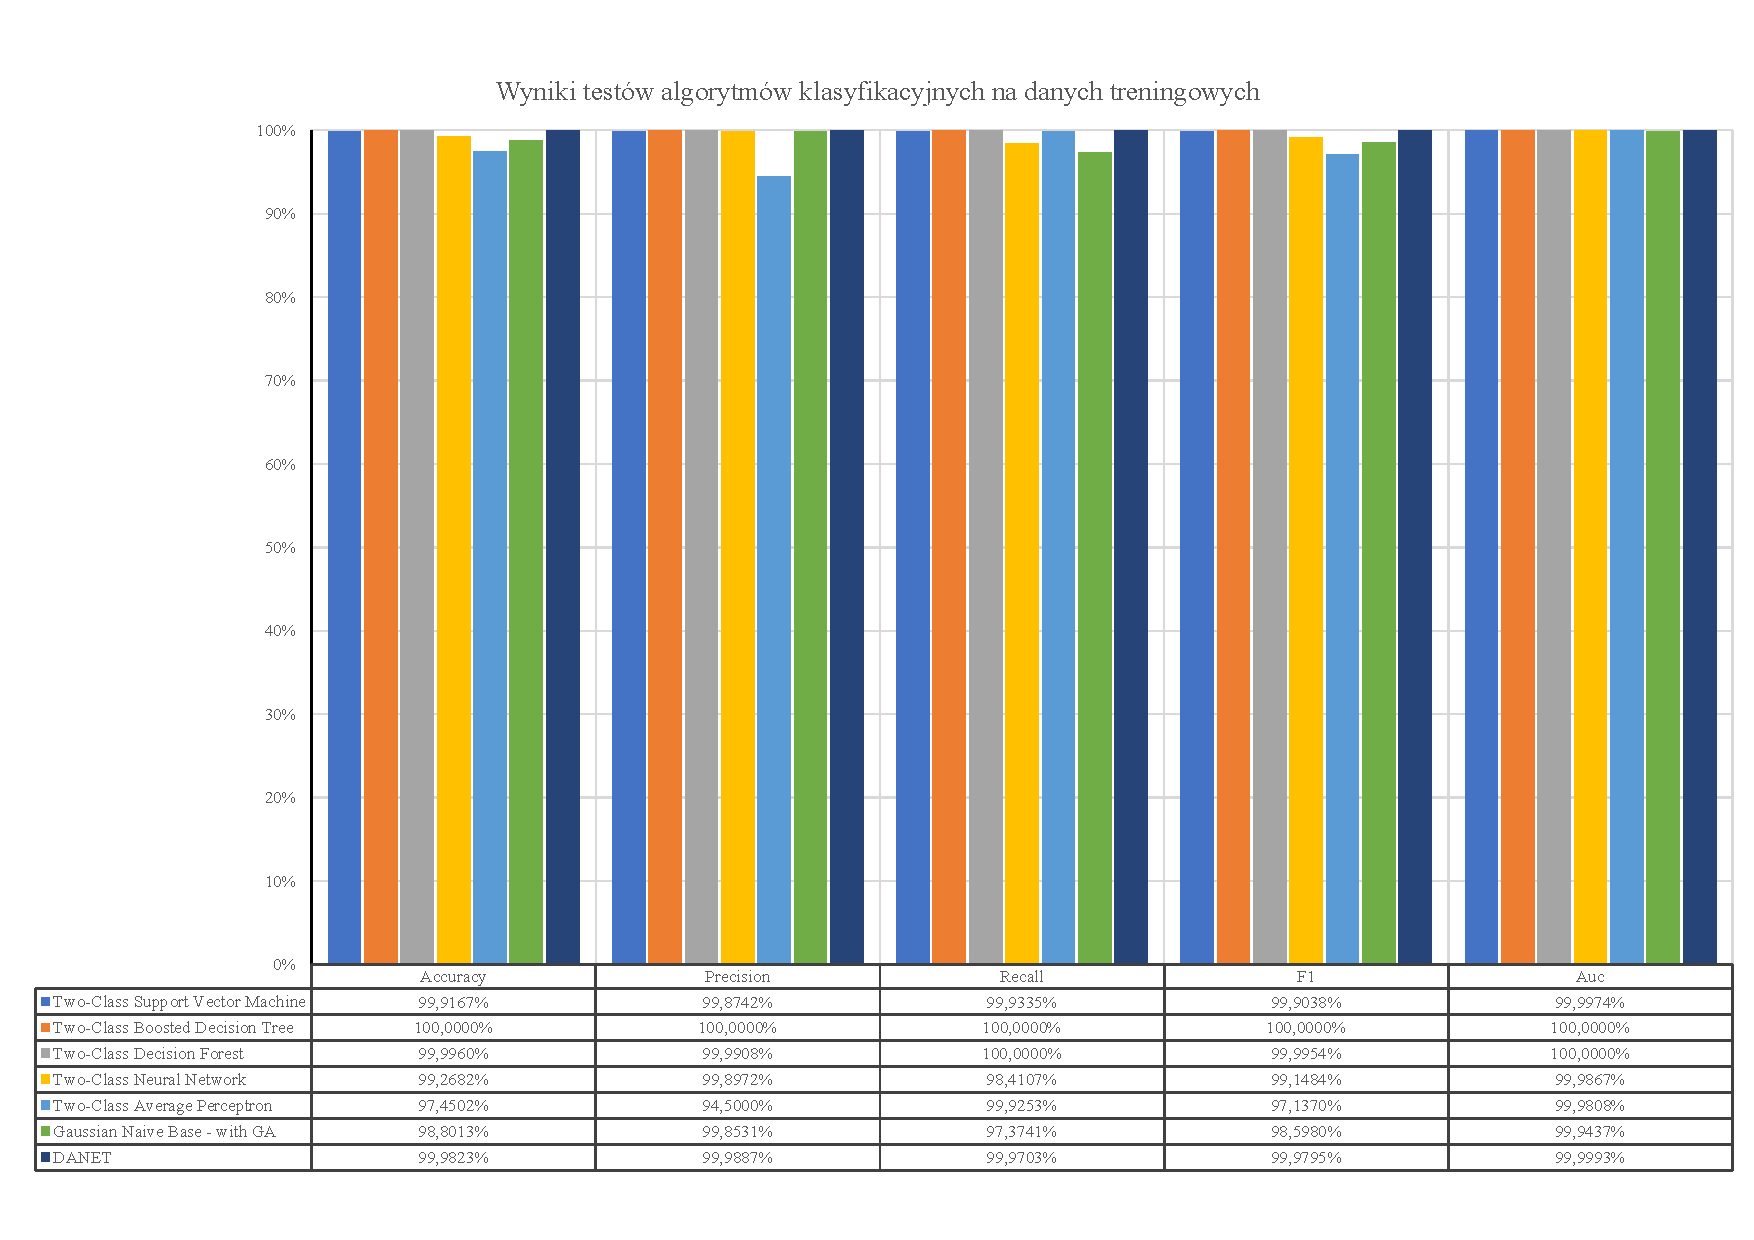
\includegraphics[height=0.8\textwidth]{images/predict_same}
        \captionsource{Wyniki testów algorytmów klasyfikacyjnych na danych treningowych}{Opracowanie własne}
        \label{fig:predict-same}
    \end{figure}
\vfill

\end{landscape}

\section{Próba badawcza}
Aby uzyskać realne wyniki podczas porównywania poszczególnych algorytmów zastosowano zbiór treningowy opisany w \refsource{tabeli}{tab:trening-data-label} oraz zbiór testowy, który zawierał 2273097 wpisów należących do klasy ''\textbf{1}'' oraz 557646 wpisów należących do klasy ''\textbf{0}'' co sumarycznie daje: 2830743 wpisów tak jak to zostało pokazane w \refsource{tabel}{tab:res-test}.

\begin{table}[H]
    \centering
    \captionsource{Liczba elementów przynależących do danej klasy w zbiorze testowym}{Opracowanie własne}
    \label{tab:res-test}
    \begin{tabular}{|c|r|} \hline
        \textbf{Klasa} & \textbf{Liczba wystąpień} \\ \hline
        1 & 2273097 \\ \hline
        0 & 557646 \\ \hline
        \textbf{Suma} & 2830743 \\ \hline
    \end{tabular}
\end{table}

Podczas analizy można zauważyć fakt, że algorytm DANet odstaje od pozostałych algorytmów w rezultatach mierzonych większością metryk. Dokładność na poziomie $19,9691\%$ pokazuje fakt, że algorytm poprawnie zaklasyfikował jedynie $565273$ wpisów. Wynik taki pokazuje, że ten algorytm jest niewystarczający do tego problemu dlatego został wykluczony z dalszych porównań.

\subsection{Dopasowanie}
Wśród pozostałych algorytmów najlepsze dopasowanie uzyskał algorytm: ''\textit{Two-Class Average Perceptron}'', którzy uzyskał wynik na poziomie $85,776\%$, zaś najgorzej poradził sobie ''\textit{Two-Class Support Vector Machine}'' uzyskując $80,3002\%$ w teście. Mimo tego te 6 algorytmó uzyskało podobne wyniki mieszczące się w granicy 3 punktów procentowych różnicy od średniego dopasowania. Algorytm autora (''\textit{Gaussian Naive Base - with GA}'') (GAGNB) uzyskał w tym teście $80,3004\%$. Wyniki zostały przedstawione w \refsource{tabeli}{tab:acc-res} oraz na \refsource{wykresie}{fig:acc-res}.

\begin{table}[H]
    \centering
    \captionsource{Wynik dopasowania algorytmów}{Opracowanie własne}
    \begin{tabular}{|l|r|} \hline
        \textbf{Algorytm} & \textbf{Wartość} \\ \hline
        Two-Class Support Vector Machine & $80,3002\%$ \\ \hline
        Two-Class Boosted Decision Tree & $83,8482\%$ \\ \hline
        Two-Class Decision Forest & $83,1725\%$ \\ \hline
        Two-Class Neural Network & $84,7332\%$ \\ \hline
        Two-Class Average Perceptron & $85,7768\%$ \\ \hline
        Gaussian Naive Base - with GA & $80,3004\%$ \\ \hline
        \end{tabular}
    \label{tab:acc-res}
\end{table}

\begin{landscape}
    \vspace*{\fill}
    \begin{figure}[H]
        \centering
        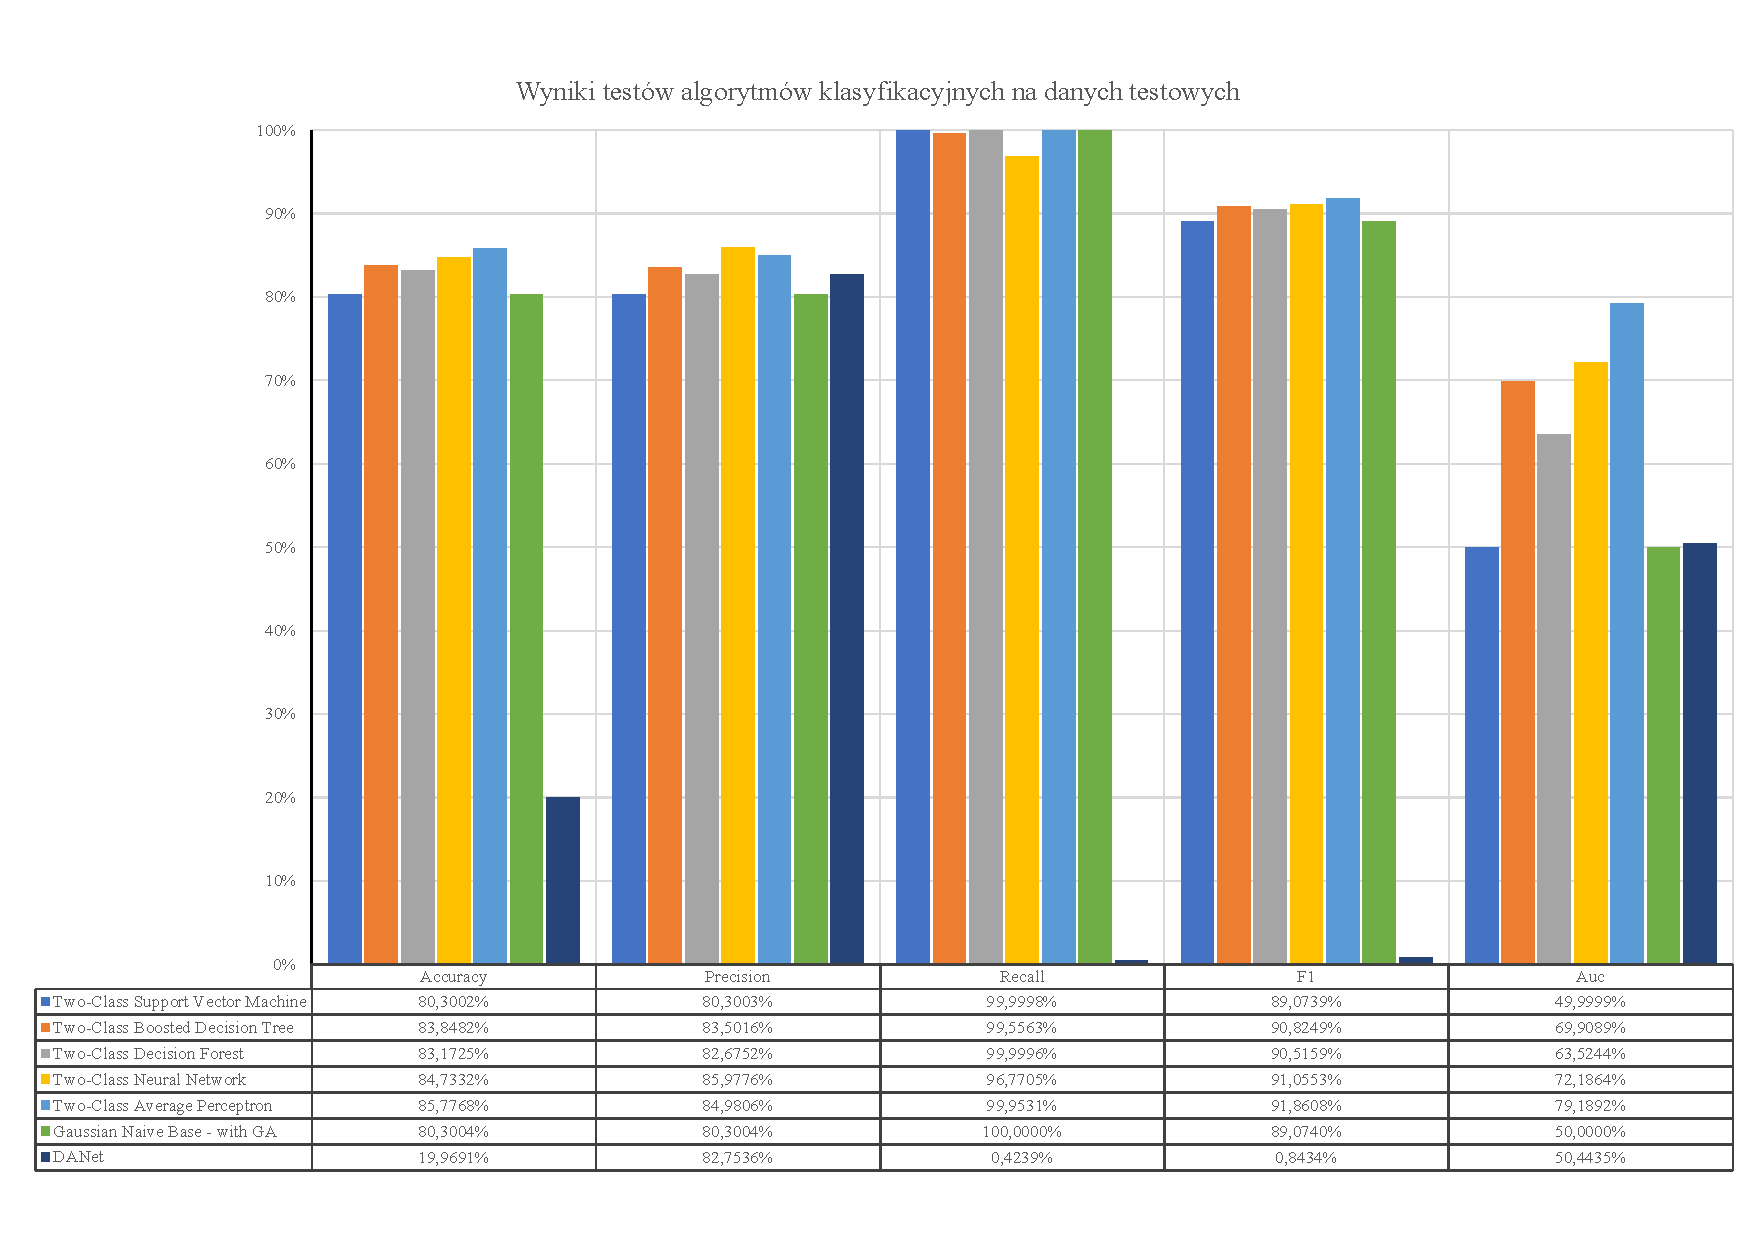
\includegraphics[height=0.8\textwidth]{images/predict_result}
        \captionsource{Wyniki testów algorytmów klasyfikacyjnych na danych testowych}{Opracowanie własne}
        \label{fig:predict-result}
    \end{figure}
    \vfill
\end{landscape}


\begin{figure}[H]
    \centering
    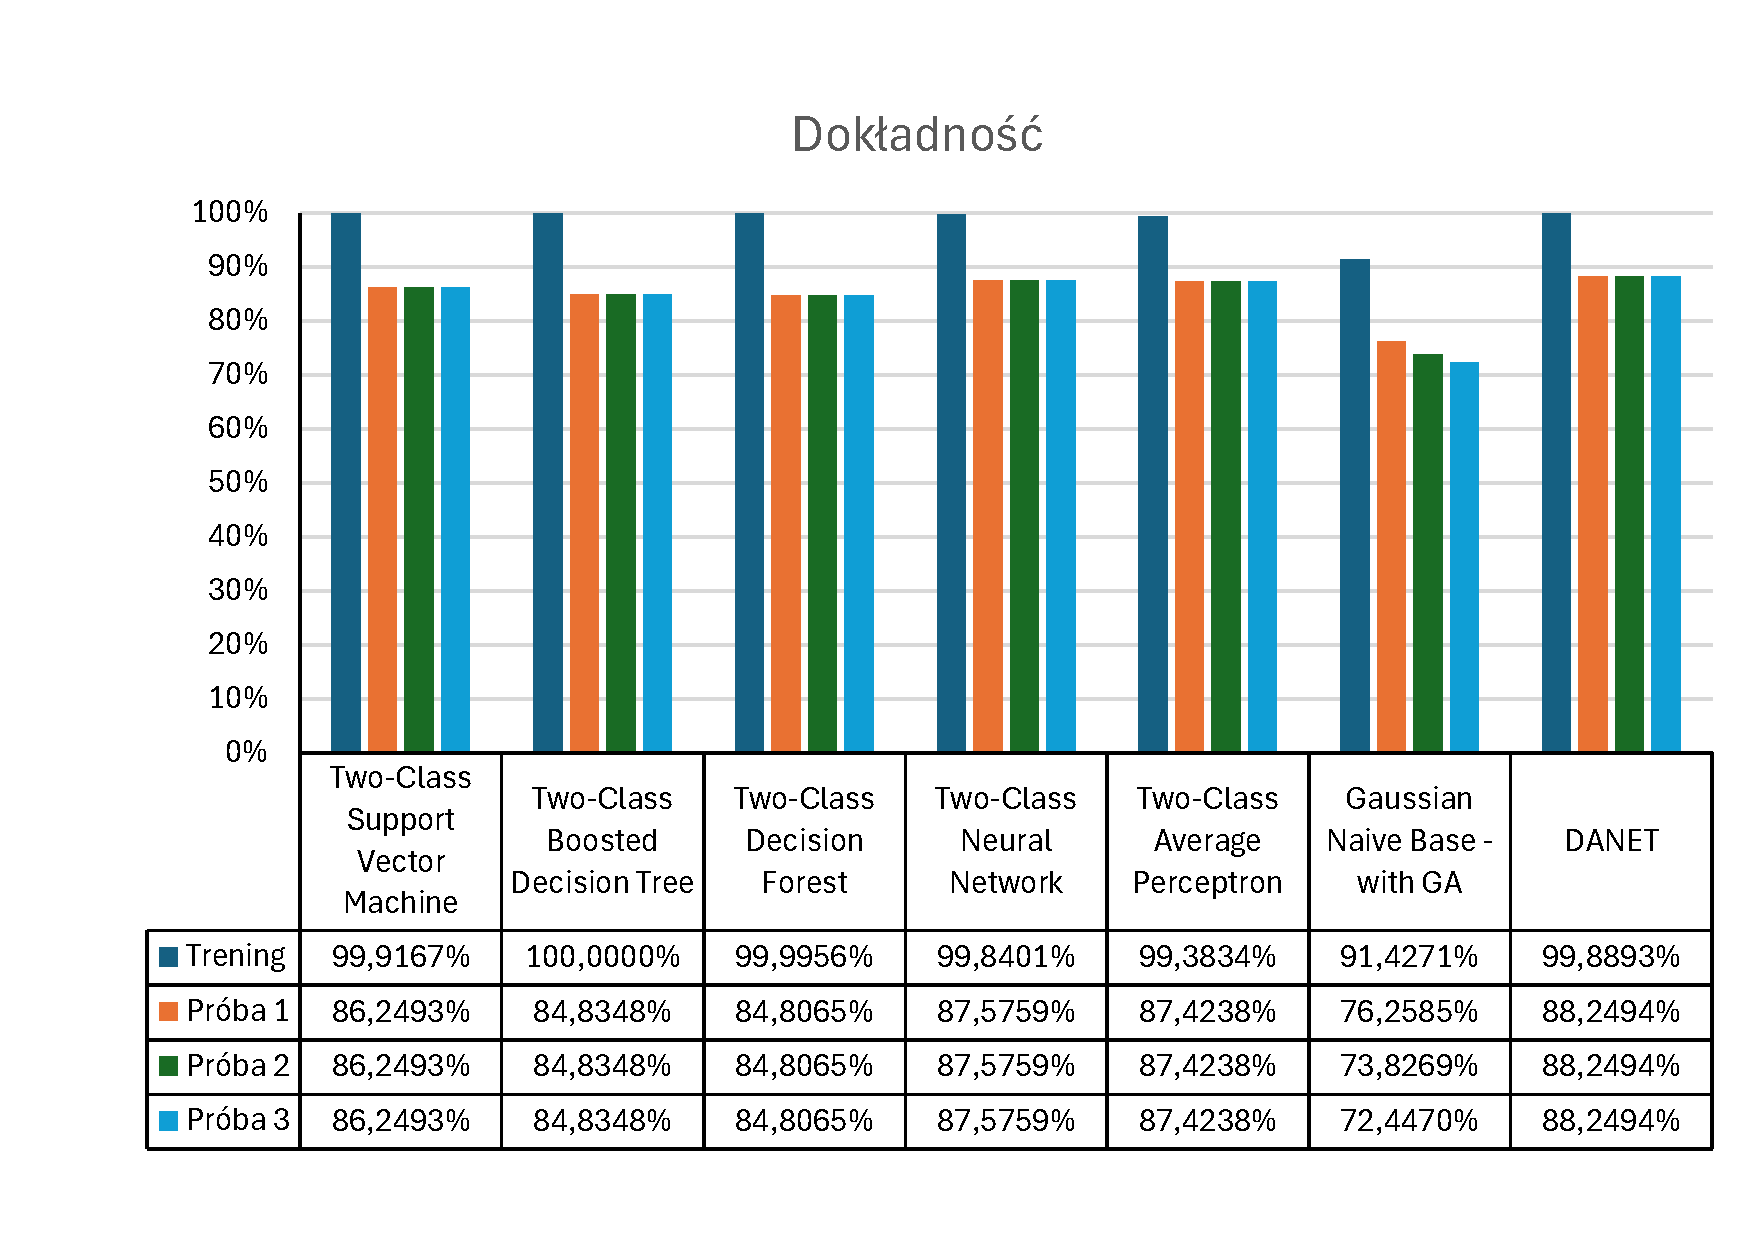
\includegraphics[width=\textwidth]{images/acc-res}
    \captionsource{Dokładność algorytmów}{Opracowanie własne}
    \label{fig:acc-res}
\end{figure}

\subsection{Precyzja}
Najlepszy wynik precyzji uzyskał algorytm ''\textit{Two-Class Neural Network}'' ($85,9776\%$) co oznacza, że najlepiej poradził sobie z dopasowaniem ruchu klasy ''\textbf{1}''. Najsłabszy wynik uzyskał ''\textit{Two-Class Support Vector Machine}'' ($80,3003\%$). GAGNB uzyskał $80,3004\%$ precyzji. Wyniki są opisane w \refsource{tabeli}{tab:acc-prec} oraz na \refsource{wykresie}{fig:acc-prec}.

\begin{table}[H]
    \centering
    \captionsource{Wynik precyzji algorytmów}{Opracowanie własne}
    \begin{tabular}{|l|r|} \hline
    \textbf{Algorytm} & \textbf{Wartość} \\ \hline
    Two-Class Support Vector Machine & $80,3003\%$ \\ \hline
    Two-Class Boosted Decision Tree & $83,5016\%$ \\ \hline
    Two-Class Decision Forest & $82,6752\%$ \\ \hline
    Two-Class Neural Network & $85,9776\%$ \\ \hline
    Two-Class Average Perceptron & $84,9806\%$ \\ \hline
    Gaussian Naive Base - with GA & $85,7768\%$ \\ \hline
    \end{tabular}
    \label{tab:acc-prec}
\end{table}

\begin{figure}[H]
    \centering
    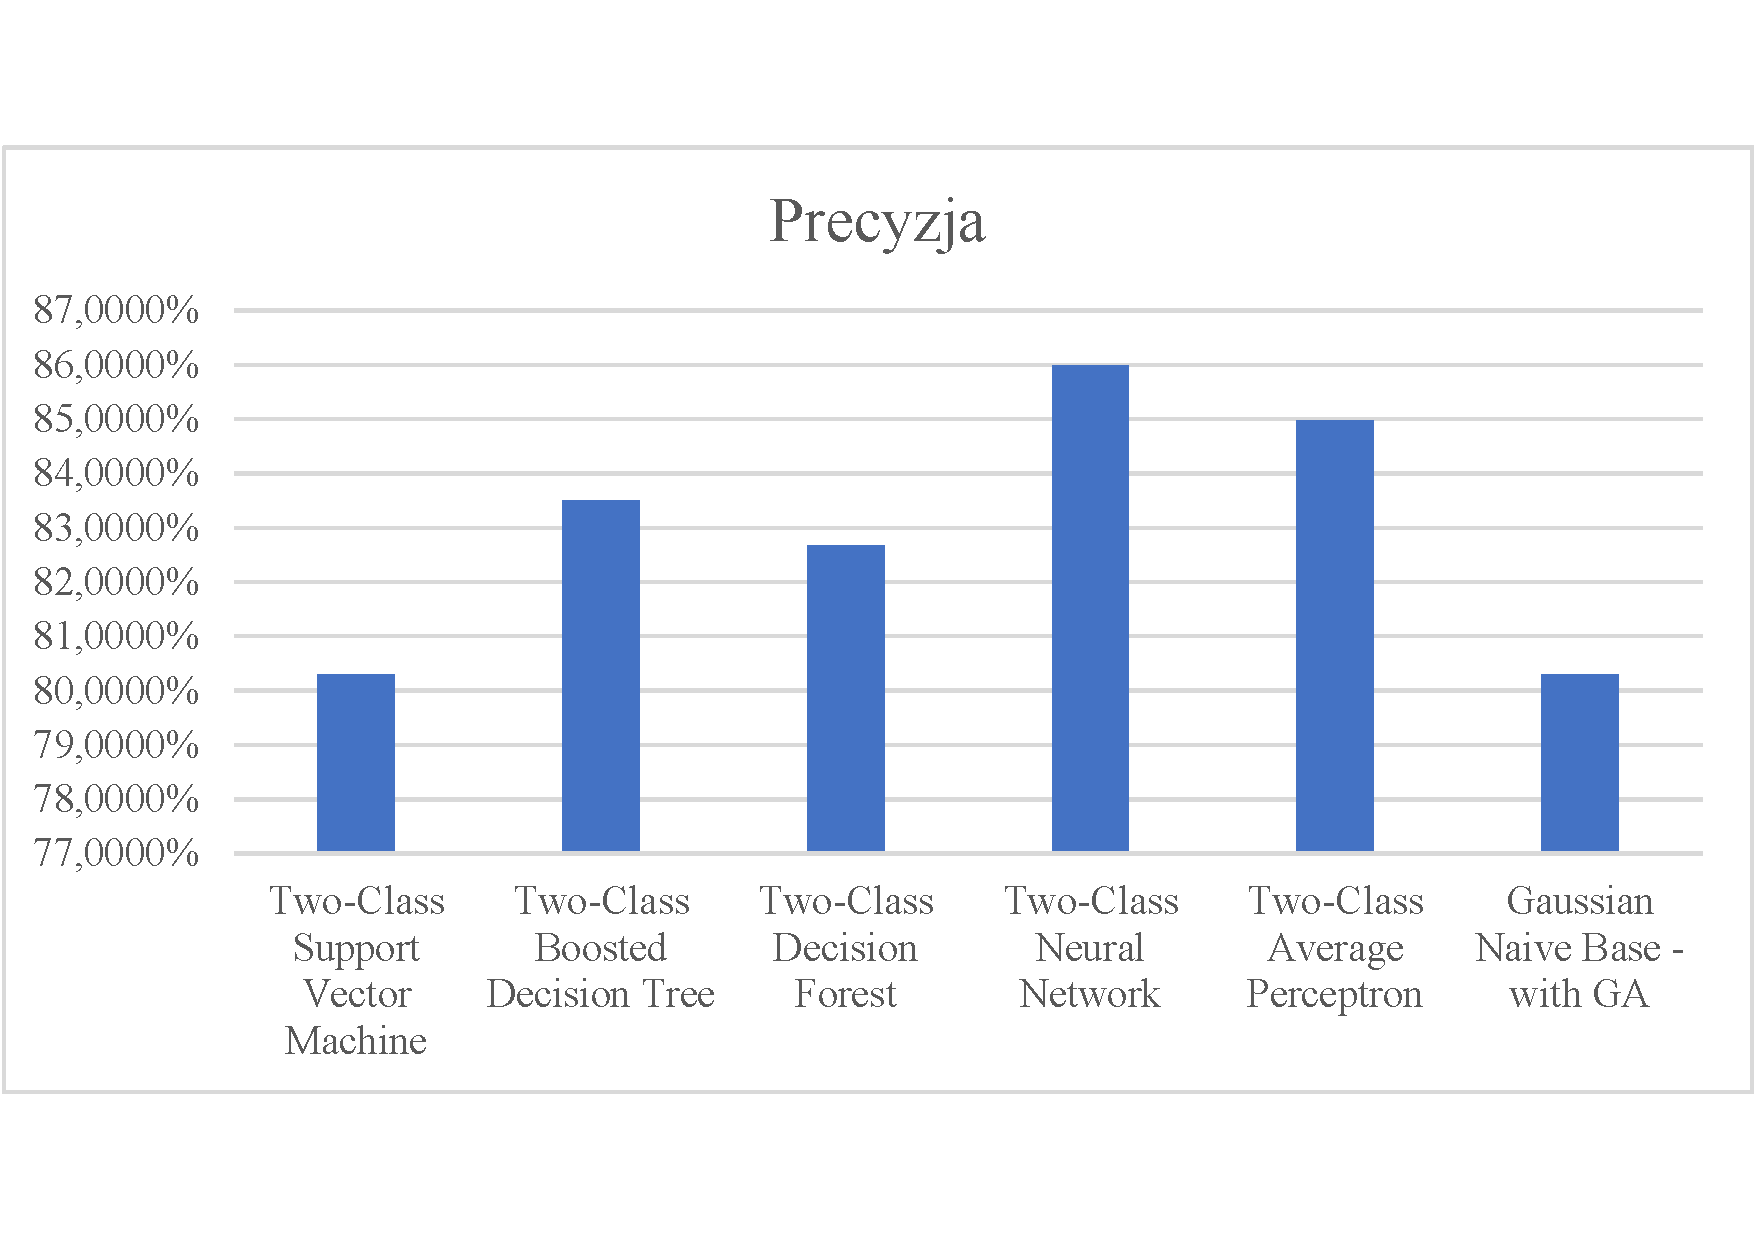
\includegraphics[width=\textwidth]{images/prec-res}
    \captionsource{Precyzja algorytmów}{Opracowanie własne}
    \label{fig:acc-prec}
\end{figure}

\subsection{Czułośc}
Wszystkie wpisy klasy ''\textbf{1}'' zostały poprawnie sklasyfikowane przez algorytm ''\textit{Gaussian Naive Base - with GA}'' ($100\%$), najsłabiej poradził sobie ''\textit{Two-Class Neural Network}'' ($96,7705\%$). Wartości zostały przedstawione w \refsource{tabeli}{tab:rec-res} oraz na \refsource{wykresie}{fig:rec-res}.

\begin{table}[H]
    \centering
    \captionsource{Wynik czułości algorytmów}{Opracowanie własne}
    \begin{tabular}{|l|r|} \hline
    \textbf{Algorytm} & \textbf{Wartość} \\ \hline
    Two-Class Support Vector Machine & $99,9998\%$ \\ \hline
    Two-Class Boosted Decision Tree & $99,5563\%$ \\ \hline
    Two-Class Decision Forest & $99,9996\%$ \\ \hline
    Two-Class Neural Network & $96,7705\%$ \\ \hline
    Two-Class Average Perceptron & $99,9531\%$ \\ \hline
    Gaussian Naive Base - with GA & $100\%$ \\ \hline
    \end{tabular}
    \label{tab:acc-rec}
\end{table}

\begin{figure}[H]
    \centering
    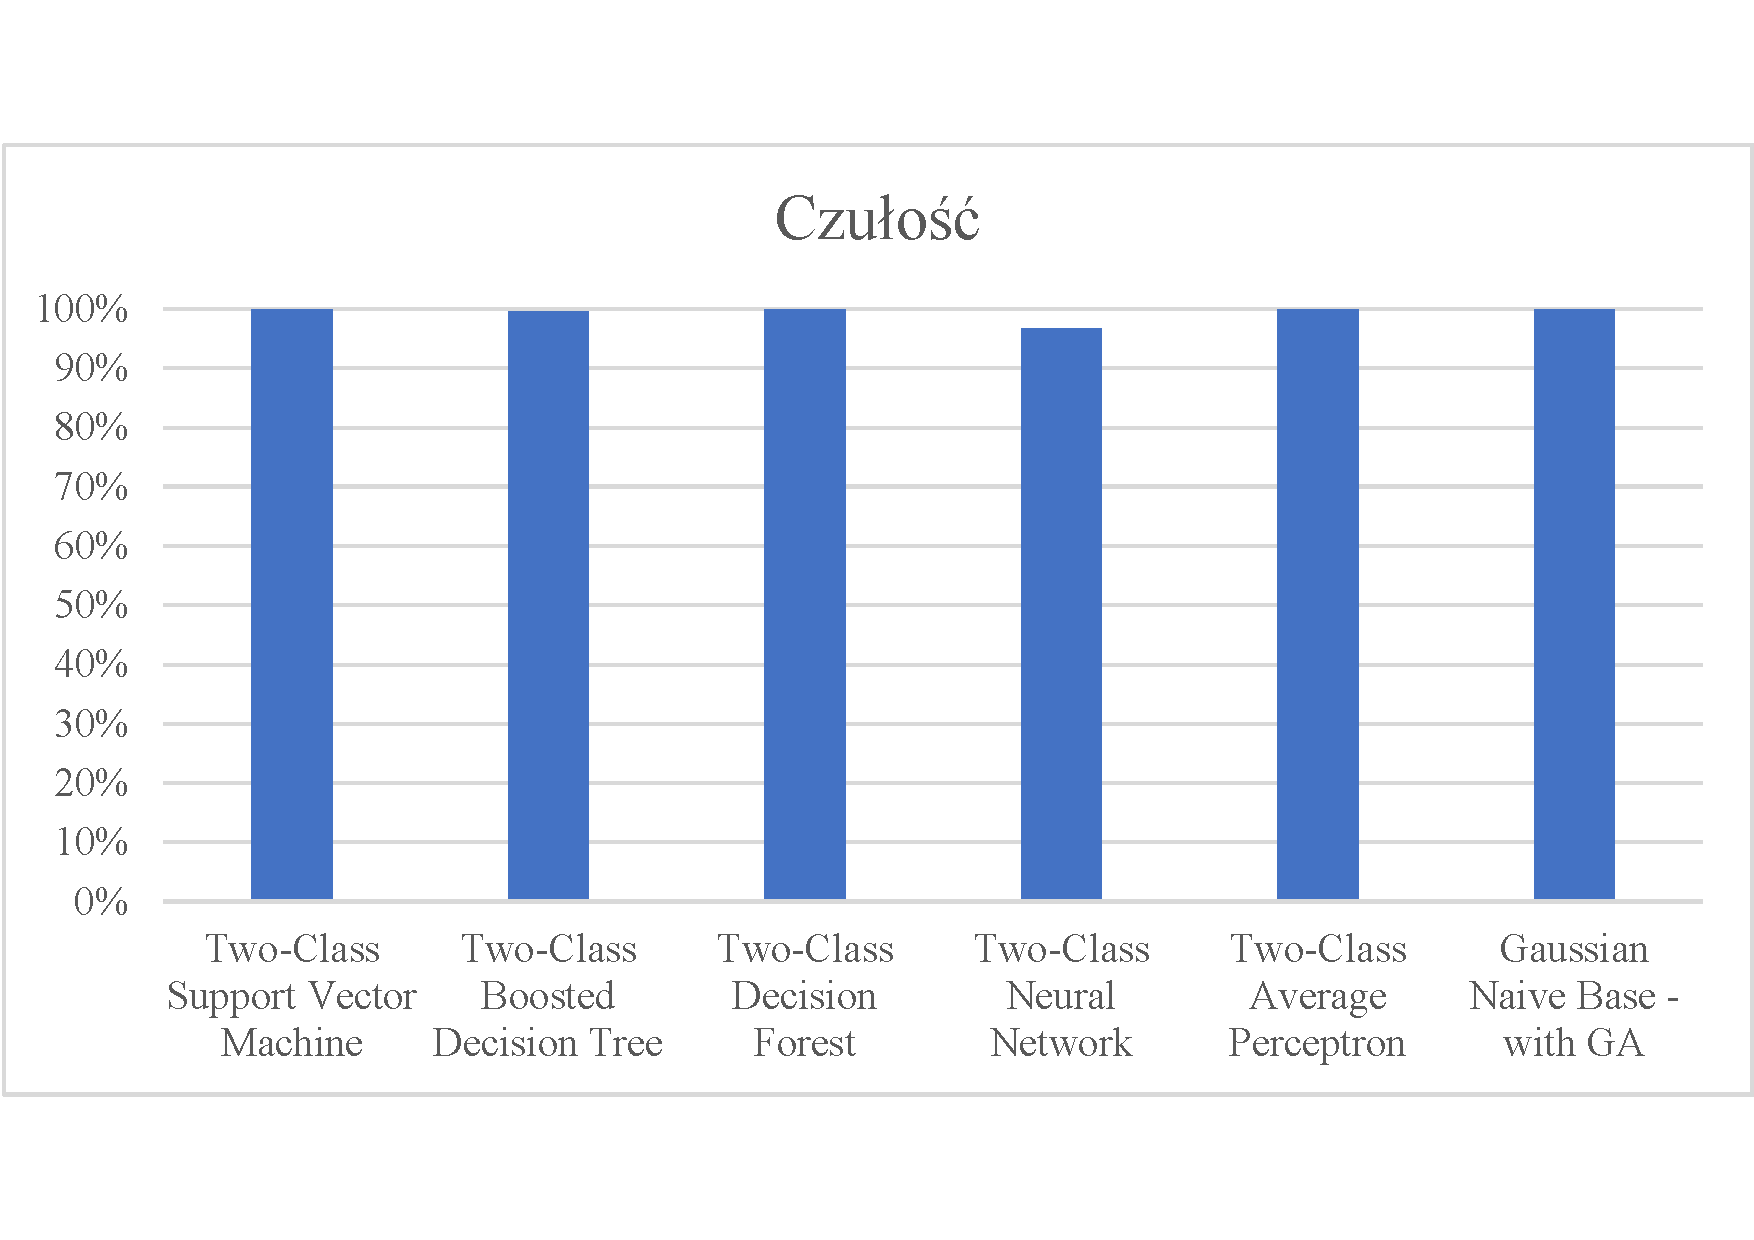
\includegraphics[width=\textwidth]{images/rec-res}
    \captionsource{Czułość algorytmów}{Opracowanie własne}
    \label{fig:rec-res}
\end{figure}

\subsection{F1}
Największą wartość F1 uzyskał ''\textit{Two-Class Average Perceptron}'' ($91,8608\%$). Najmniejszą uzyskał ''\textit{Two-Class Support Vector Machine}'' ($89,0739\%$). GAGNB w tym teście uzyskał $89,0740\%$. Wyniki zostały przedstawione w \refsource{tabeli}{tab:acc-f1} oraz na \refsource{wykresie}{fig:f1-res}.

\begin{table}[H]
    \centering
    \captionsource{Wynik F1 algorytmów}{Opracowanie własne}
    \begin{tabular}{|l|r|} \hline
    \textbf{Algorytm} & \textbf{Wartość} \\ \hline
    Two-Class Support Vector Machine & $89,0739\%$ \\ \hline
    Two-Class Boosted Decision Tree & $90,8249\%$ \\ \hline
    Two-Class Decision Forest & $90,5159\%$ \\ \hline
    Two-Class Neural Network & $91,0553\%$ \\ \hline
    Two-Class Average Perceptron & $91,8608\%$ \\ \hline
    Gaussian Naive Base - with GA & $89,0740\%$ \\ \hline
    \end{tabular}
    \label{tab:acc-f1}
\end{table}

\begin{figure}[H]
    \centering
    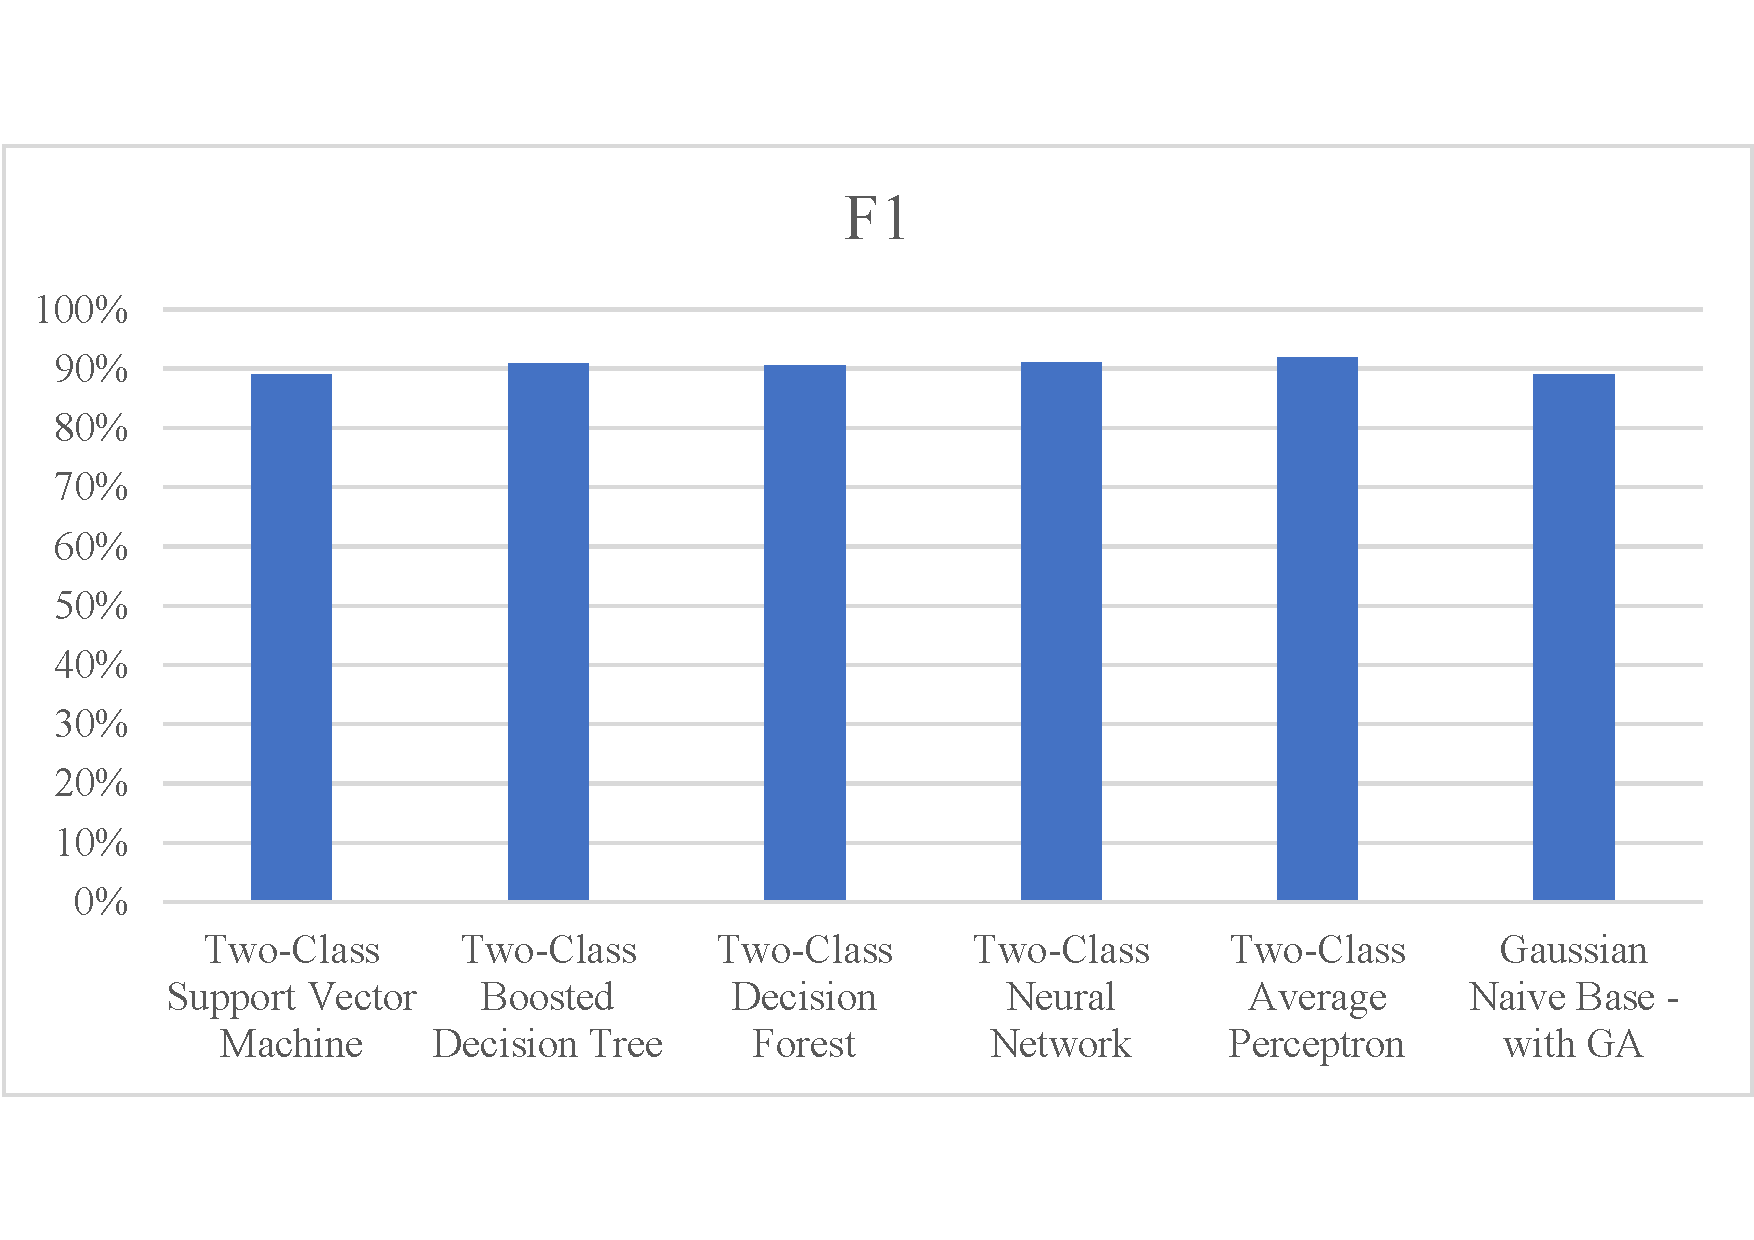
\includegraphics[width=\textwidth]{images/f1-res}
    \captionsource{F1 algorytmów}{Opracowanie własne}
    \label{fig:f1-res}
\end{figure}

\subsection{AUC}
Analizując wynik AUC, można zauważyć, że najlepsza sprawność również uzyskał algorytm ''\textit{Two-Class Average Perceptron}'' ($79,1292\%$). Najgorszy algorytm to znów algorytm wykorzystujący SVM ($49,9999\%$), wynik wskazał na to, że algorytm ten miał niższą sprawność niż próba losowa. W tym teście sprawność algorytmu GAGNB wyniosła $50\%$. Wyniki przedstawiono w \refsource{tabeli}{tab:acc-auc} oraz na \refsource{wykresie}{fig:auc-res}.

\begin{table}[H]
    \centering
    \captionsource{Wynik czułości algorytmów}{Opracowanie własne}
    \begin{tabular}{|l|r|} \hline
    \textbf{Algorytm} & \textbf{Wartość} \\ \hline
    Two-Class Support Vector Machine & $49,9999\%$ \\ \hline
    Two-Class Boosted Decision Tree & $69,9089\%$ \\ \hline
    Two-Class Decision Forest & $63,5244\%$ \\ \hline
    Two-Class Neural Network & $72,1864\%$ \\ \hline
    Two-Class Average Perceptron & $79,1892\%$ \\ \hline
    Gaussian Naive Base - with GA & $50\%$ \\ \hline
    \end{tabular}
    \label{tab:acc-auc}
\end{table}

\begin{figure}[H]
    \centering
    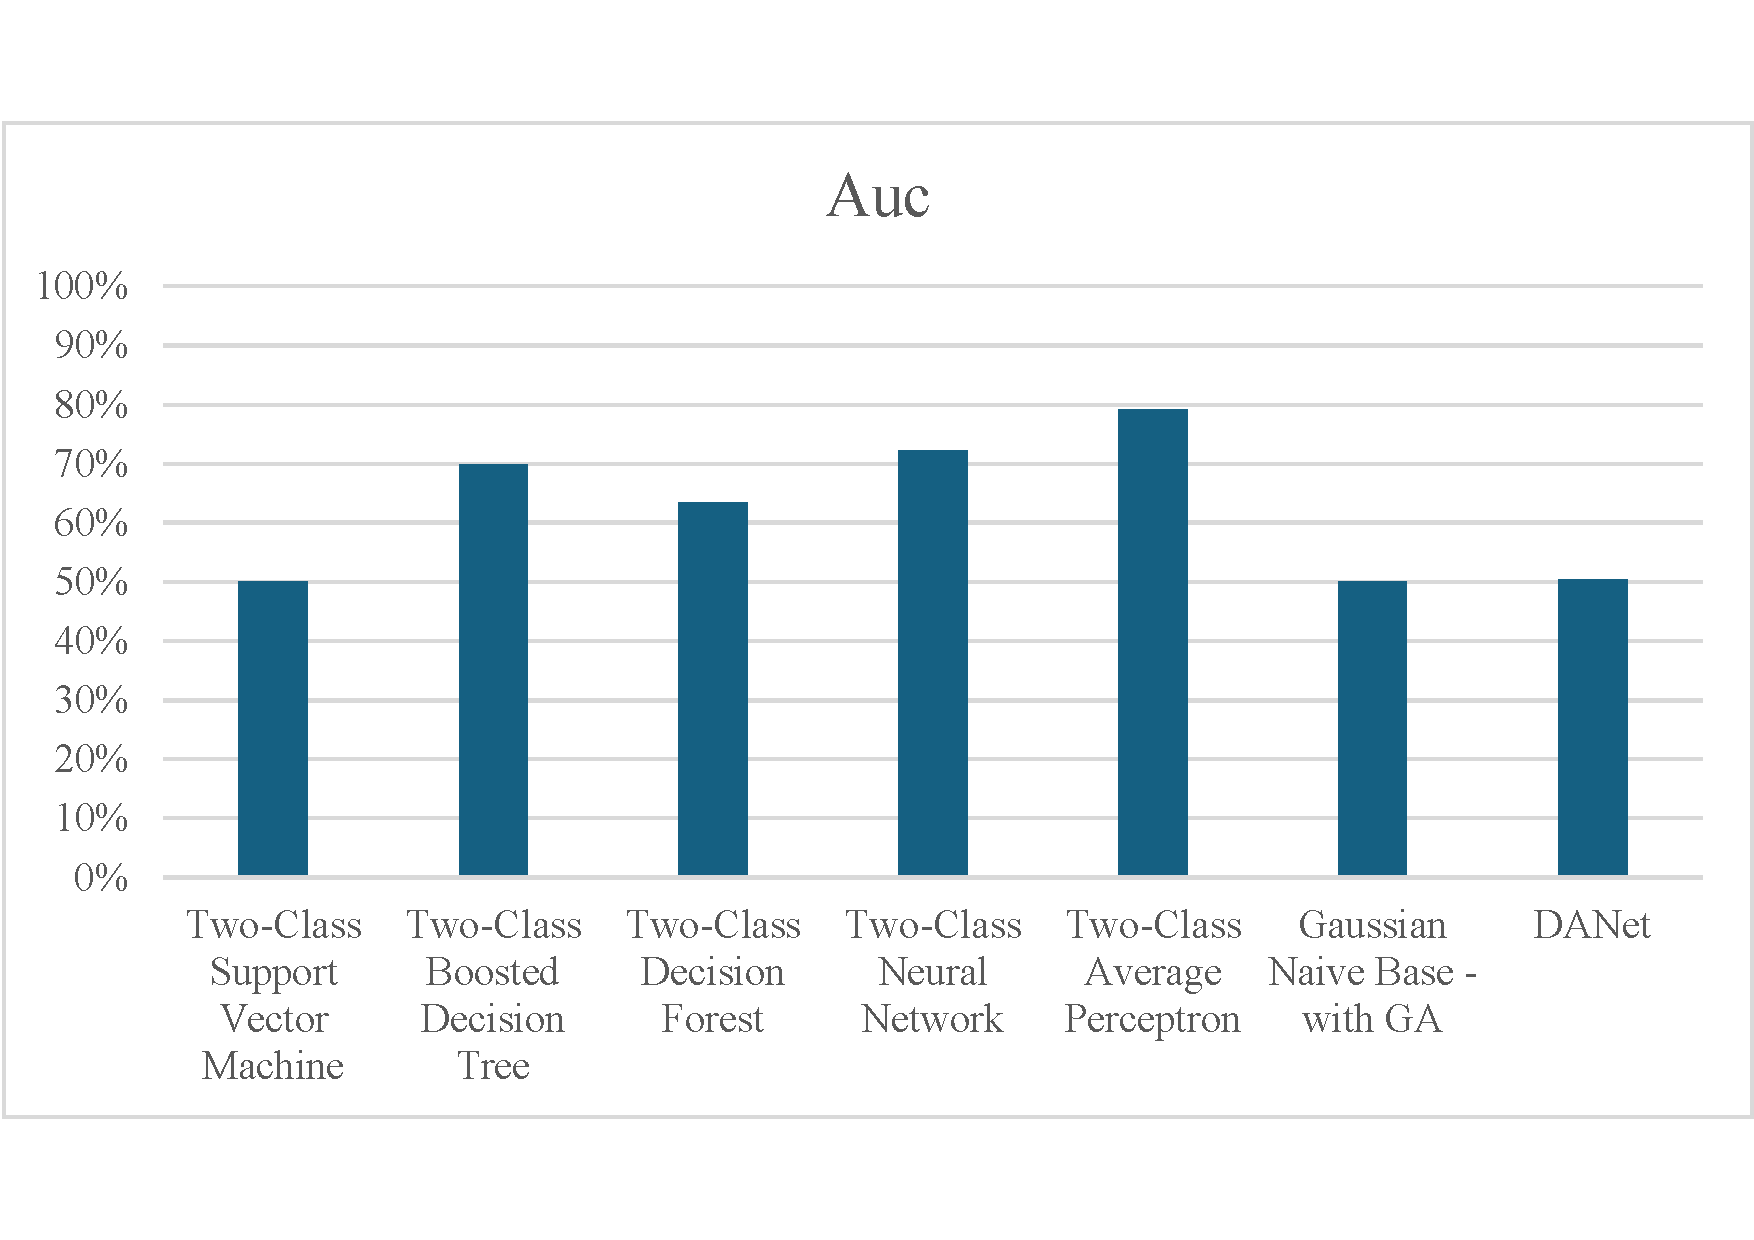
\includegraphics[width=\textwidth]{images/auc-res}
    \captionsource{AUC algorytmów}{Opracowanie własne}
    \label{fig:auc-res}
\end{figure}

\section{Wnioski}

Microsoft Wyszedł na przeciw potrzebom użytkowników dlatego przygotował zestaw prekonfigurowanych algorytmów klasyfikacyjnych, dzięki czemu możliwości narzędzia Azure ML pozwalają na odpowiadanie na konkretne potrzeby przy relatywnie niewielkich kosztach. Jednakże to nie oznacza, że tworzenie autorskich rozwiązań mija się z celem. Jak ukazano na \refsource{wykresie}{fig:predict-result} autorskie rozwiązania również mają rację bytu. Wykorzystanie połączenia algorytmu genetycznego i klasyfikatora naiwnego Bayesa z rozkładem normalnym pozwala na uzyskanie zbliżonych wyników co algorytmu utworzone przez giganta technologicznego. Różnica około 5 punktó procentywych między najlepszym algorytmem a algorytmem GAGNB ukazuje niewielką różnicę w jakości algorytmu. Dodatkowo wciąż trudno korzysta się z rozwiązań takich jak DANet, któe są nieprzetestowe na różnorakich zbiorach lecz na tych wcześniej specjalnie spreparowanych.
\\ \\
Dodatkowo korzystanie z tego typu prostych rozwiązań autorskich pozwala na prototypownie rozwiązań biznesowych opartych o klasyfikację danych. Samo wykorzystanie algorytmu genetycznego z algorytmem GNB umożliwia skupienie się na tworzenie ugólnego rozwiązania bez wcześniejszej znajomości zbioru oraz korzystając z programów lokalnie nie ponosząc kosztów wykorzystania platformy chmurowej. Kolejnym atutem utworzonego przez autora rozwiązania jest zmniejszenie kosztów lokalnego użytkowania poprzez zmniejszenie wymiarowości zbioru danych do klasyfikacji poprzez wykorzystanie jedynei wytypowanych kolumn.
\\ \\
Doświadczenie to ukazuje, że wciąż należy próbować tworzyć wydajniejsze i dokładniejsze rozwiązania, lecz nie zaprzecza faktu iż rozwiązania ogólnie dostępne są na bardzo wysokim poziomie. Uzyskano dokładność z zakresu $[80\%, 85\%]$ przy czym plik testowy był 12 krotnie większy od pliku treningowego.


	\chapter{Podsumowanie}
Niniejsza praca magisterska miała na celu, wykonanie porównania algorytmów klasyfikacyjnych dostarczonych przez platformę Azure, wraz z GAGNB oraz algorytmem DANet.\ Wśród autorskich algorytmów znajdywał się algorytm opracowany przez autora pracy magisterskiej - \textit{Gaussian Naive Bayes - with GA}.\ Miało to na celu sprawdzenie, czy tworzenie autorskich rozwiązań nakierowanych na problem będzie opłacalne w dobie gotowych rozwiązań.
\\ \\
W pracy dokonano przeglądu literaturowego związanego zagadnieniem uczenia maszynowego oraz z podejściem low-code/no-code.\ Dzięki temu wybrano narzędzie Machine Learning Studio znajdujące się na platformie Microsoft Azure. \ Microsoft wyszedł naprzeciw potrzebom użytkowników, przygotowując zestaw prekonfigurowanych algorytmów klasyfikacyjnych.\ Możliwości narzędzia Azure ML pozwalają na tworzenie wysokoskalowalnych rozwiązań z zakresu uczenia maszynowego przy relatywnie niskich kosztach.\ Jednakże mogą wystąpić specyficzne wymagania biznesowe albo prawne, które nie będą pozwalały na zastosowanie zewnętrznych narzędzi chmurowych.\ Takim przykładem są strategiczne dane państwowe, których wyciek za granicą może grozić poważnym zagrożeniem z zewnątrz.\ W przypadku systemów wykrywania intruzów zasadne jest stosowanie autorskich rozwiązań, które nie są znane opinii publicznej.\ Takie działanie chroni przed nieautoryzowanym dostępem do sieci komputerowej oraz do danych wrażliwych.
\\ \\
Konkurencyjność rozwiązań autorskich przedstawiono na \refsource{wykresie}{fig:predict-result}.\ Wykorzystanie połączenia algorytmu genetycznego i klasyfikatora naiwnego Bayesa z rozkładem normalnym pozwala na uzyskanie zbliżonych wyników do algorytmu utworzonych przez Microsoft.\ Różnica około 5 punktów procentowych między najlepszym algorytmem a algorytmem \textit{Gaussian Naive Bayes - with GA} ukazuje niewielką różnicę w jakości algorytmu.\ Częstą wadą autorskich rozwiązań jest ich nakierowanie na konkretny zestaw danych.\ Zostało to pokazane podczas wykorzystania algorytmu DANet, który dobrze sklasyfikował dane związane z m.in. chorobami serca~\cite{Chen2022}.\ Algorytm ten jednakże błędnie skategoryzował dane związane z ruchem sieciowym.
\\ \\
Dodatkowo korzystanie z tego typu prostych rozwiązań autorskich pozwala na prototypownie rozwiązań biznesowych opartych o klasyfikację danych.\ Zastosowanie algorytmu \textit{GAGNB} nie wymaga wcześniejszej znajomości zbioru danych.\ Pozwala na lokalne korzystanie z programu do klasyfikacji, bez ponoszenia kosztów wykorzystania platformy chmurowej.\ Kolejnym atutem tego algorytmu jest zmniejszenie kosztów lokalnego użytkowania.\ Co zostało spowodowane zmniejszeniem wymiarowości zbioru danych do klasyfikacji poprzez wykorzystanie jedynie wytypowanych kolumn.
\\ \\
Stworzony projekt jest jedynie silnikiem klasyfikacyjnym, który pozwala na wytrenowanie i wyłonienie najlepszego algorytmu do klasyfikacji danych.\ Dzięki możliwościom platformy Azure ML stworzenie całego środowiska testowego jest relatywnie tanie i nie wymaga wielu wyspecjalizowanych umiejętności.\ Bazując na wynikach i najlepszym klasyfikatorze, można utworzyć odpowiednie przepływy służące do klasyfikacji danych wejściowych.\ Dostęp do nich może odbywać się za pomocą utworzonych Punktów Dostępowych \trans{ang. Endpoints}.\ Dzięki punktom dostępowym możliwa jest komunikacja za pomocą protokołu HTTPS \trans{ang. Hyper Text Transfer Protocol Secure} i komunikacja typu REST \textit{(ang. Representative State Transfer)}.
\\ \\
Utworzony w ten sposób punkt dostępu może zostać wykorzystany w klasyfikacji ruchu sieciowego w niewielkich aplikacjach z dostępem do internetu.\ Pozwoliłoby to na realizację analizy danych w chmurze, co mogłoby przyspieszyć cały proces oraz utworzyć pojedyncze źródło prawdy dla wielu instancji aplikacji.\ A wykorzystanie dodatkowo konteneryzacji, którą zapewnia platforma Azure, cały proces mógłby zostać zoptymalizowany pod kątem wydajnościowym i lokalizacyjnym.\ Pojedyncze źródło prawdy jest zaletą wykorzystania ,,\textit{zewnętrznego}'' klasyfikatora, ponieważ zapewnia jednakowe wyniki klasyfikacji w poszczególnych instancjach samej aplikacji instalowanej na wielu urządzeniach.\ Pozwala to również na lepsze dostrajanie całego procesu, a wykorzystanie kolejnych wersji przepływów umożliwia utrzymywanie kopii zapasowych poszczególnych rozwiązań.\ Umożliwia to na przykład cofnięcie wersji klasyfikatora w przypadku wykrycia nieprawidłowości w obecnym modelu.


	\renewcommand*{\listfigurename}{Wykaz rysunków}
	\renewcommand*{\listtablename}{Wykaz tabel}
	\listoffigures
	\clearpage
	\listoftables

	\printbibliography

\end{document}
